\section{Results}

\subsection{Descriptive statistics}

The 78,396 patients attended 111 hospitals with admissions ranging from 267 to 1,414, and thrombolysis rate ranging from 24\% to 67\%. Of the 43,152 patients who do not receive thrombolysis (and not thrombectomy), 18\% has mRS 0, 28\% have mRS 1, 23\% have mRS 2, 20\% have mRS 3, 16\% have mRS 4, 9\% have mRS 5, and 17\% have mRS 6 at discharge. Of the 32,497 patients who receive thrombolysis (and not thrombectomy), 15\% has mRS 0, 21\% have mRS 1, 18\% have mRS 2, 16\% have mRS 3, 12\% have mRS 4, 5\% have mRS 5, and 13\% have mRS 6 at discharge.

%%%%%%%%%%%%%%%%%%%%%% FEATURE SELECTION %%%%%%%%%%%%%%%%%%%%%%%%%%%%
\subsection{Feature selection}

We selected 7 features for all subsequent work. The features, in order of selection were:

\begin{enumerate}
    \item Prior disability level: Disability level (mRS) before stroke
    \item Stroke severity: Stroke severity (NIHSS) on arrival
    \item Stroke team: Hospital attended
    \item Age: Age (as middle of 5 year age bands)
    \item Onset to thrombolysis time: Time from onset to receiving thrombolysis (minutes). Set to 9,999 if did not receive thrombolysis.
    \item Any afib diagnosis: Patient has a diagnosis of atrial fibrillation (either previously diagnosed or new)
    \item Precise onset known: Onset time recorded is precise time (not a best estimate)
\end{enumerate}

A model using these 7 features was able to provide 99.1\% of the accuracy obtained when all 57 features were used (ROC-AUC: 0.796 vs 0.803). These 7 features were largely independent of each other. Correlations between the 6 features were measured (excluding stroke team). All r-squared were less than 0.05 except (a) prior disability level and age (r-squared 0.14) and (b) prior disability level and stroke severity (r-squared 0.07).

%%%%%%%%%%%%%%%%%%%%%% ACCURACY %%%%%%%%%%%%%%%%%%%%%%%%%%%%

\subsection{Model accuracy}

ROC-AUC was 0.796 (0.001 standard deviation across the 5 k-folds). Classification accuracy across the seven mRS outcomes was 41.1\% (0.002 standard deviation across the 5 k-folds). Accuracy to within one mRS category was 72.4\% (0.002 standard deviation across the 5 k-folds).  

All subsequent work described used the first k-fold split (80\% data used for training the models, and 20\% used for test results).

%%%%%%%%%%%%%%%%%%%%%% WATERFALL PLOTS %%%%%%%%%%%%%%%%%%%%%%%%%%%%

\subsection{Individual patient SHAP values}

For an example patient with mRS 2 at discharge, based on their feature values the model predicts their probability distribution across the seven target classes (figure \ref{fig:results_waterfall}). The prediction is the class with the highest probability. This example patient has a correct prediction of mRS 2 at discharge. SHAP values show how each feature value contributes to the log odds of having that level of disability at discharge, which are shown in an individual waterfall plot per target class (the seven other plots in figure \ref{fig:results_waterfall}). For each possible mRS level, the SHAP model starts with a base prediction (unique for each target class), before feature values are taken into account. The combination of this patient having a low prior disability (mRS 2) and a mild stroke severity (NIHSS 2) is important for increasing the predicted likelihood of a mRS 2 at discharge, and for reducing the predicted likelihood of the other six mRS levels.

\begin{figure}[!h]
  \centering   
 {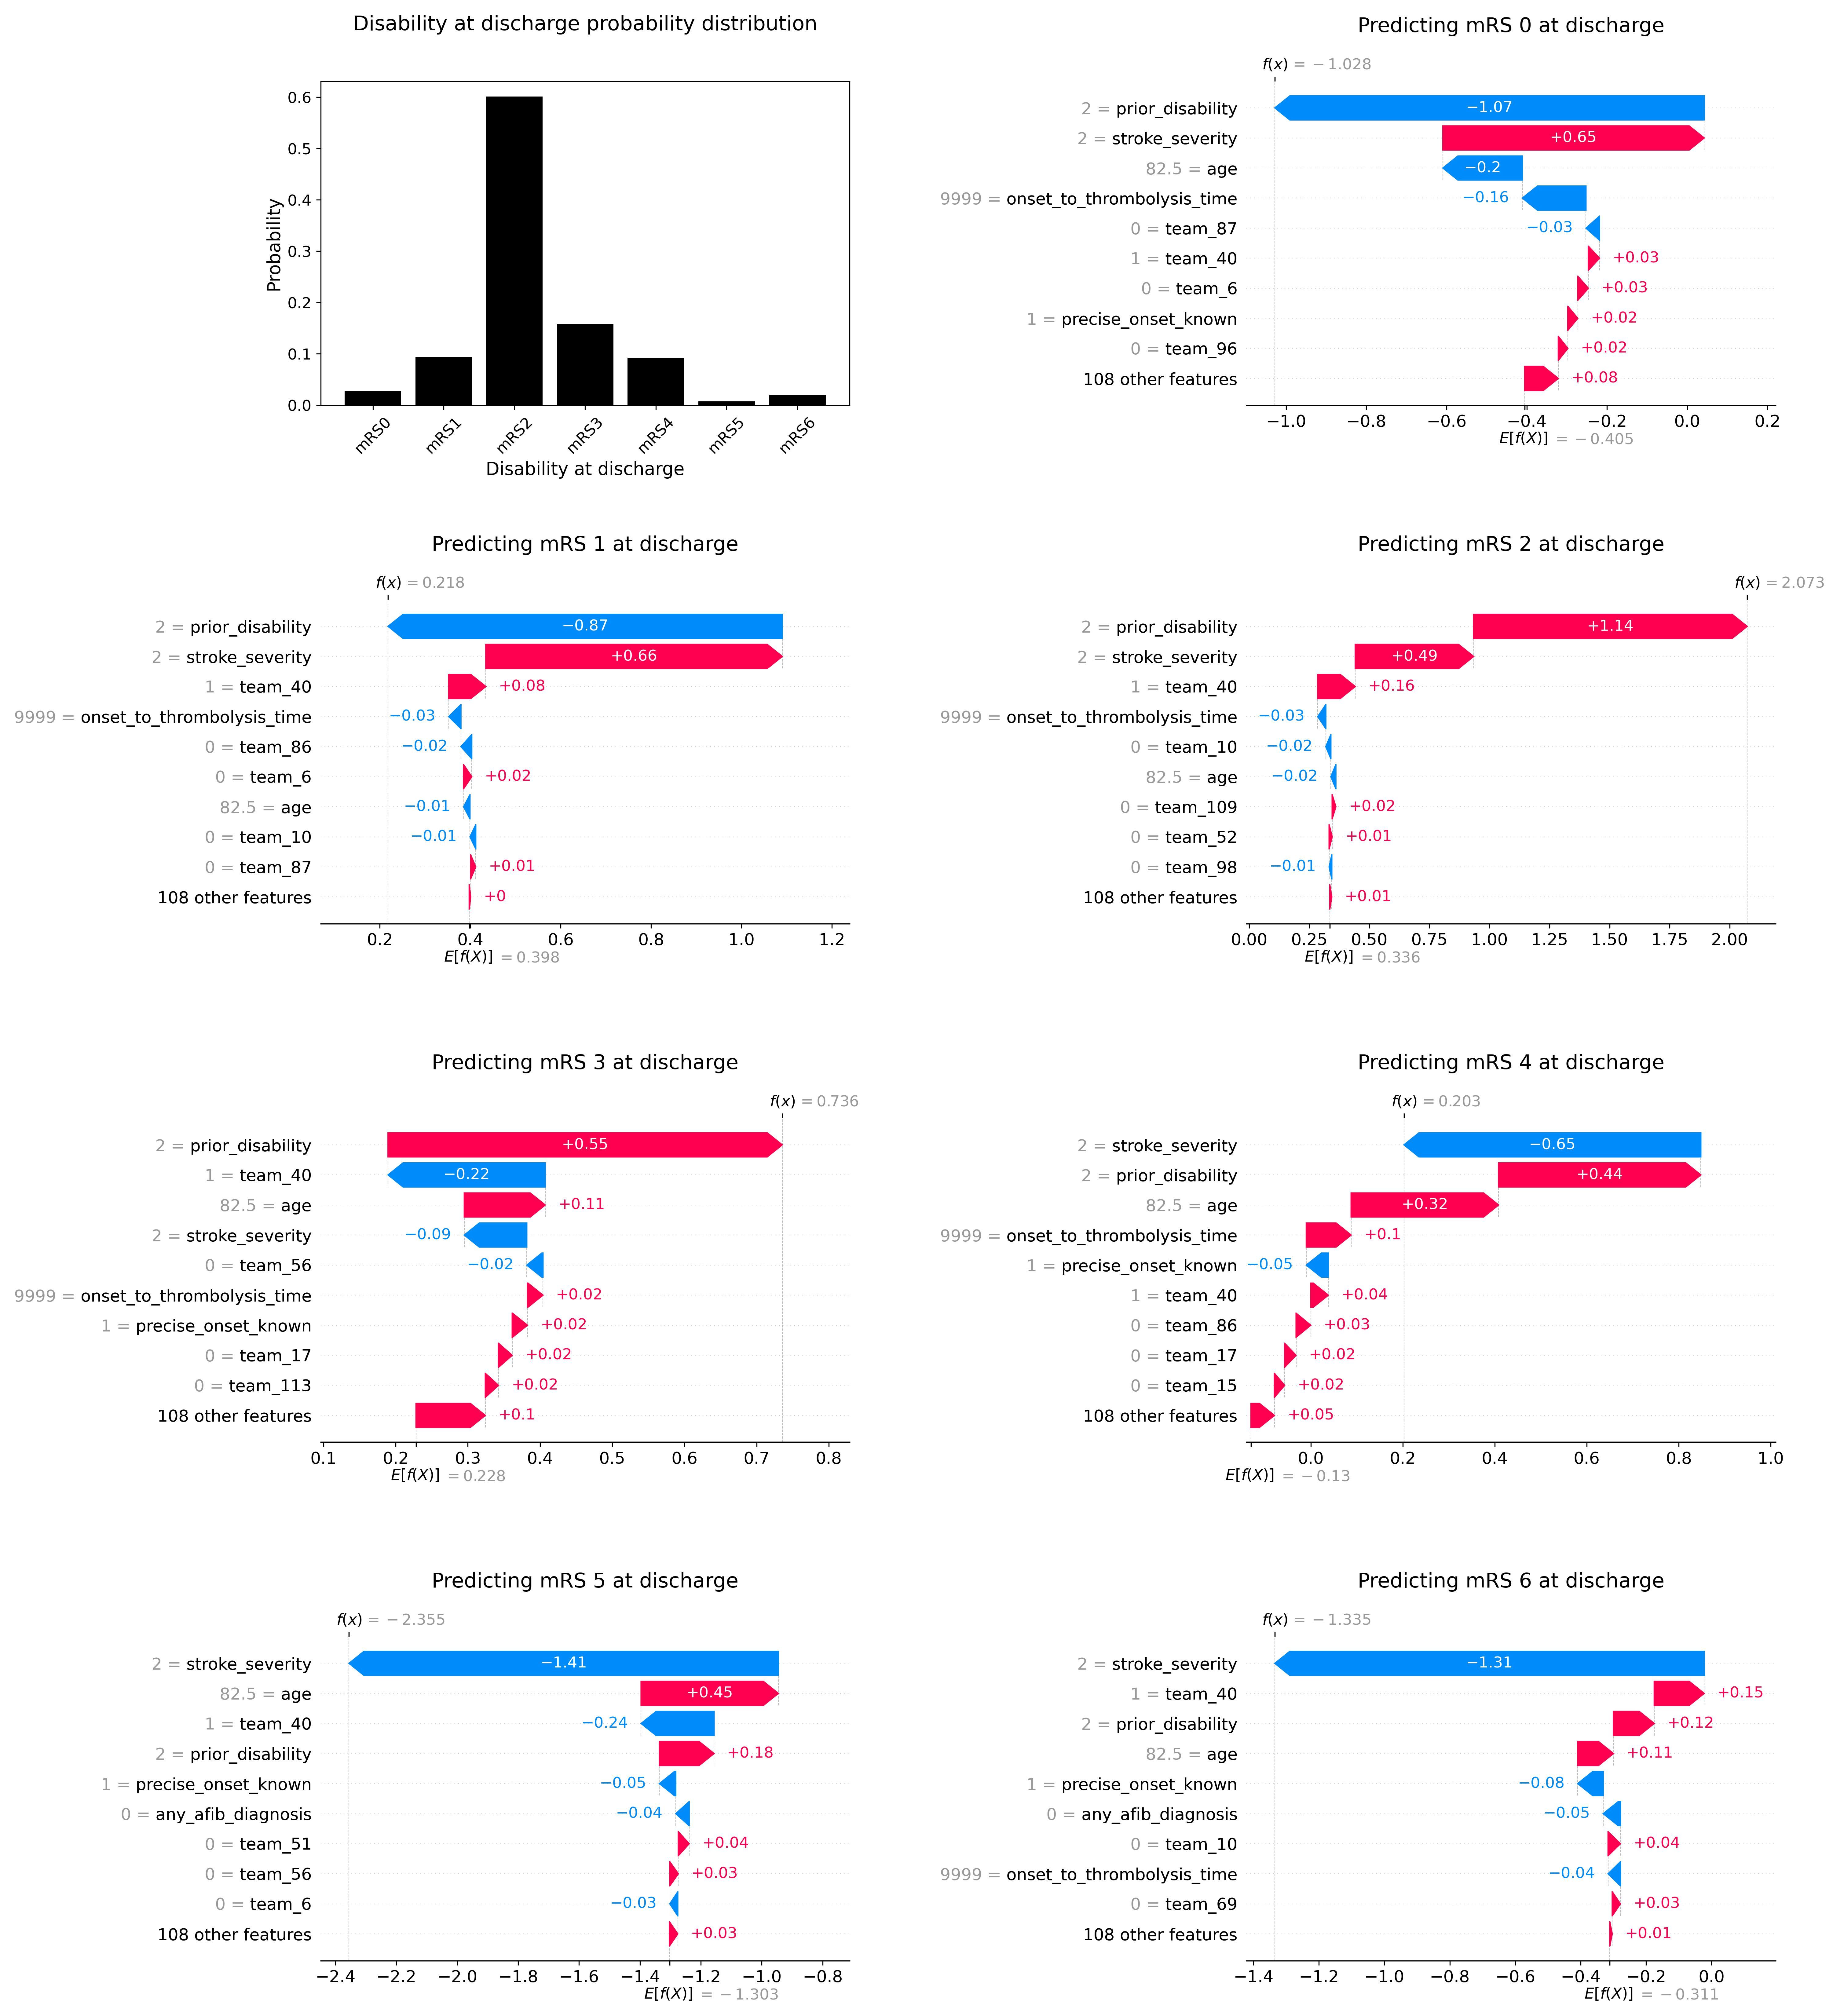
\includegraphics[width=1\linewidth]
{./images/042_xgb_7_features_5fold_probability_distribution_with_individual_waterfall_plots.jpg}}
  \caption{An example prediction for an individual patient (discharged mRS 2) showing the predicted probability of being discharged at each mRS level and waterfall plots showing the influence of each feature on the predicted likelihood of a single patient having each level of mRS at discharge. Each waterfall plot shows the SHAP base value, $E[f(X)$] (which is the same for all patient predictions for that mRS level), and the SHAP values for each of the input feature values. The sum of base and features SHAP values equates to the overall log likelihood for the patient being that mRS score at discharge, $f(x)$.}
  \label{fig:results_waterfall}
\end{figure}

%%%%%%%%%%%%%%%%%%%%%% POPULATION SHAP %%%%%%%%%%%%%%%%%%%%%%%%%%%%

\subsection{Influences on best and worst outcomes across a patient cohort}

In order to understand general characteristics affecting outcomes, we have shown how patient feature values, and stroke team attended, affected the likelihood of having the best (mRS 0) or worst (mRS 6) outcomes (figure \ref{fig:shap_outcome_model}) across 15,680 test patients (which were not used to train the model). Feature values that contributed to the best outcome on discharge (mRS 0) were no prior disability, milder stroke, earlier thrombolysis, younger, no atrial fibrillation diagnosis, and precisely known stroke onset time. Feature values that contributed to the worst outcome on discharge (mRS 6) were higher prior disability, more severe stroke, later or no thrombolysis, older, diagnosis of atrial fibrillation, and an imprecisely known onset time. The hospital attended also affected outcome predictions, with a  larger contribution from the attended hospital contribution for mRS 0, rather than mRS 6, at discharge. 


\begin{figure}
    \centering
    \begin{subfigure}{.5\textwidth}
      \centering
      \captionsetup{width=.9\linewidth}
      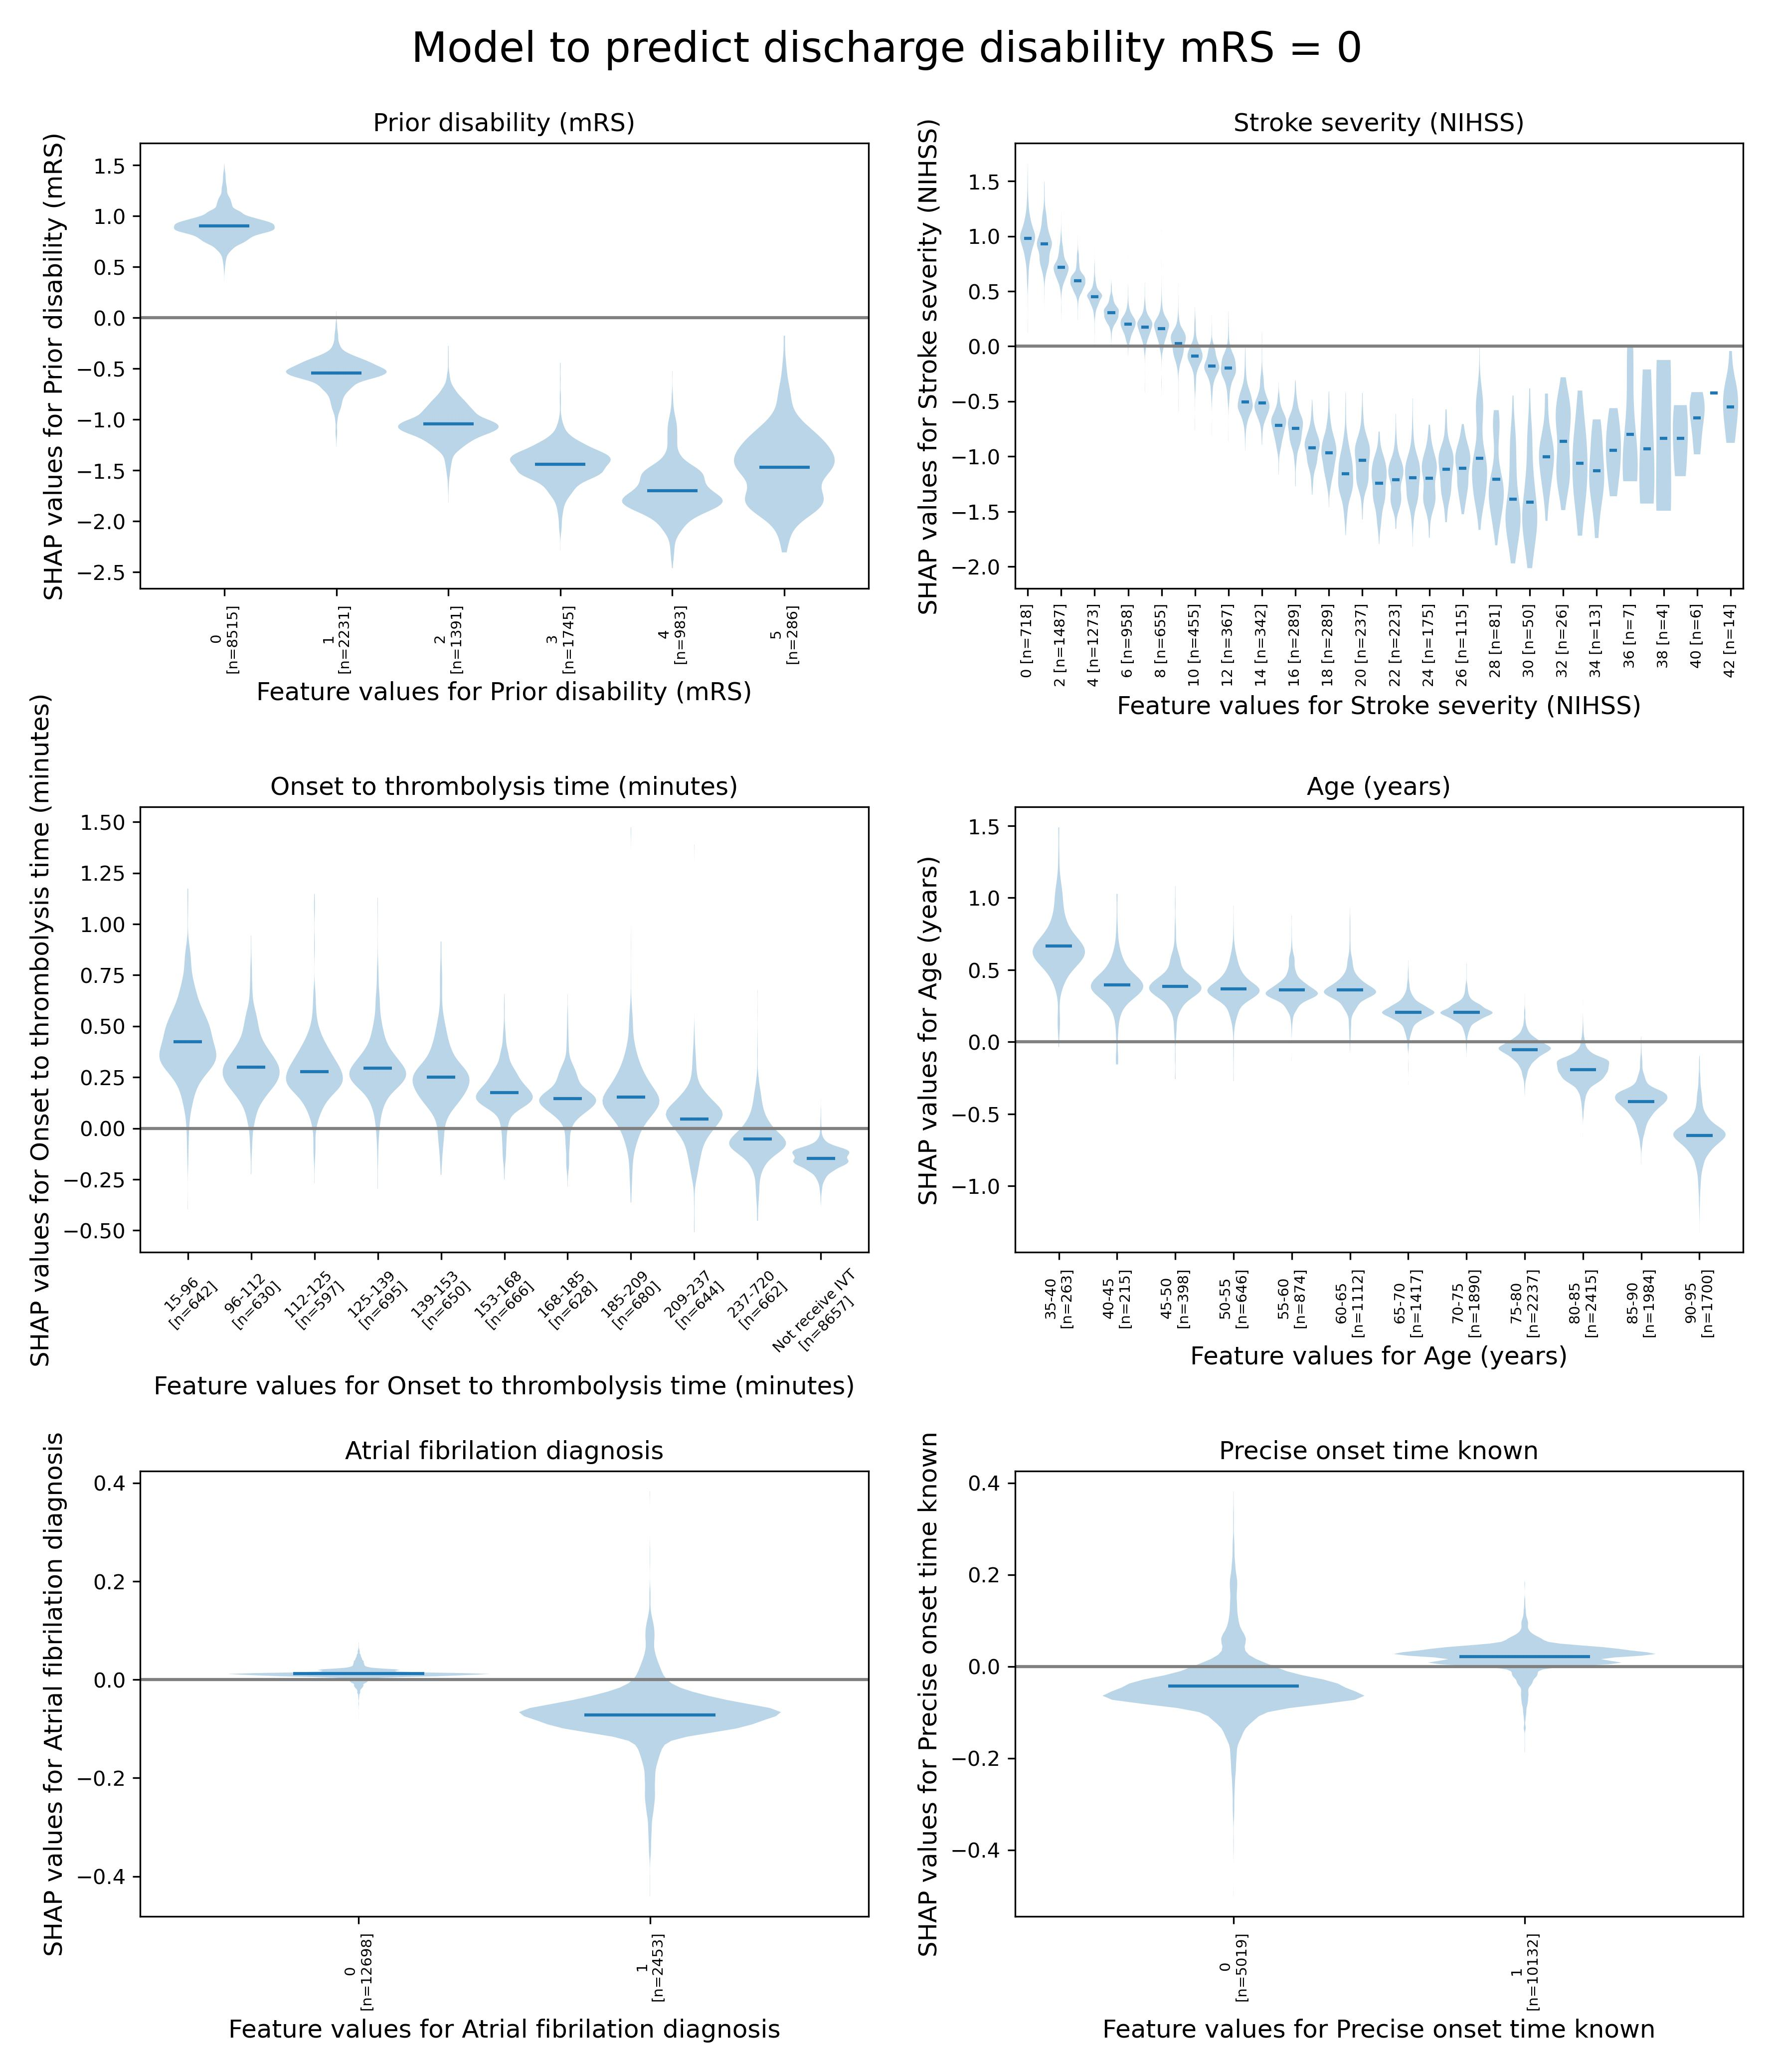
\includegraphics[trim={0 0 0 1.2cm}, clip, width=0.95\linewidth]      {./images/053_xgb_7_features_1fold_thrombolysis_shap_violin_all_features_for_mRS0}\\
      %{./images/053_xgb_7_features_1fold_999999_thrombolysis_shap_violin_all_features_for_mRS0}\\
%      \caption{SHAP values for the likelihood of no disability on discharge (mRS 0)}
%      \label{fig:mrs_violin}
    \end{subfigure}%ults
    \begin{subfigure}{.5\textwidth}
      \centering
      \captionsetup{width=.9\linewidth}
      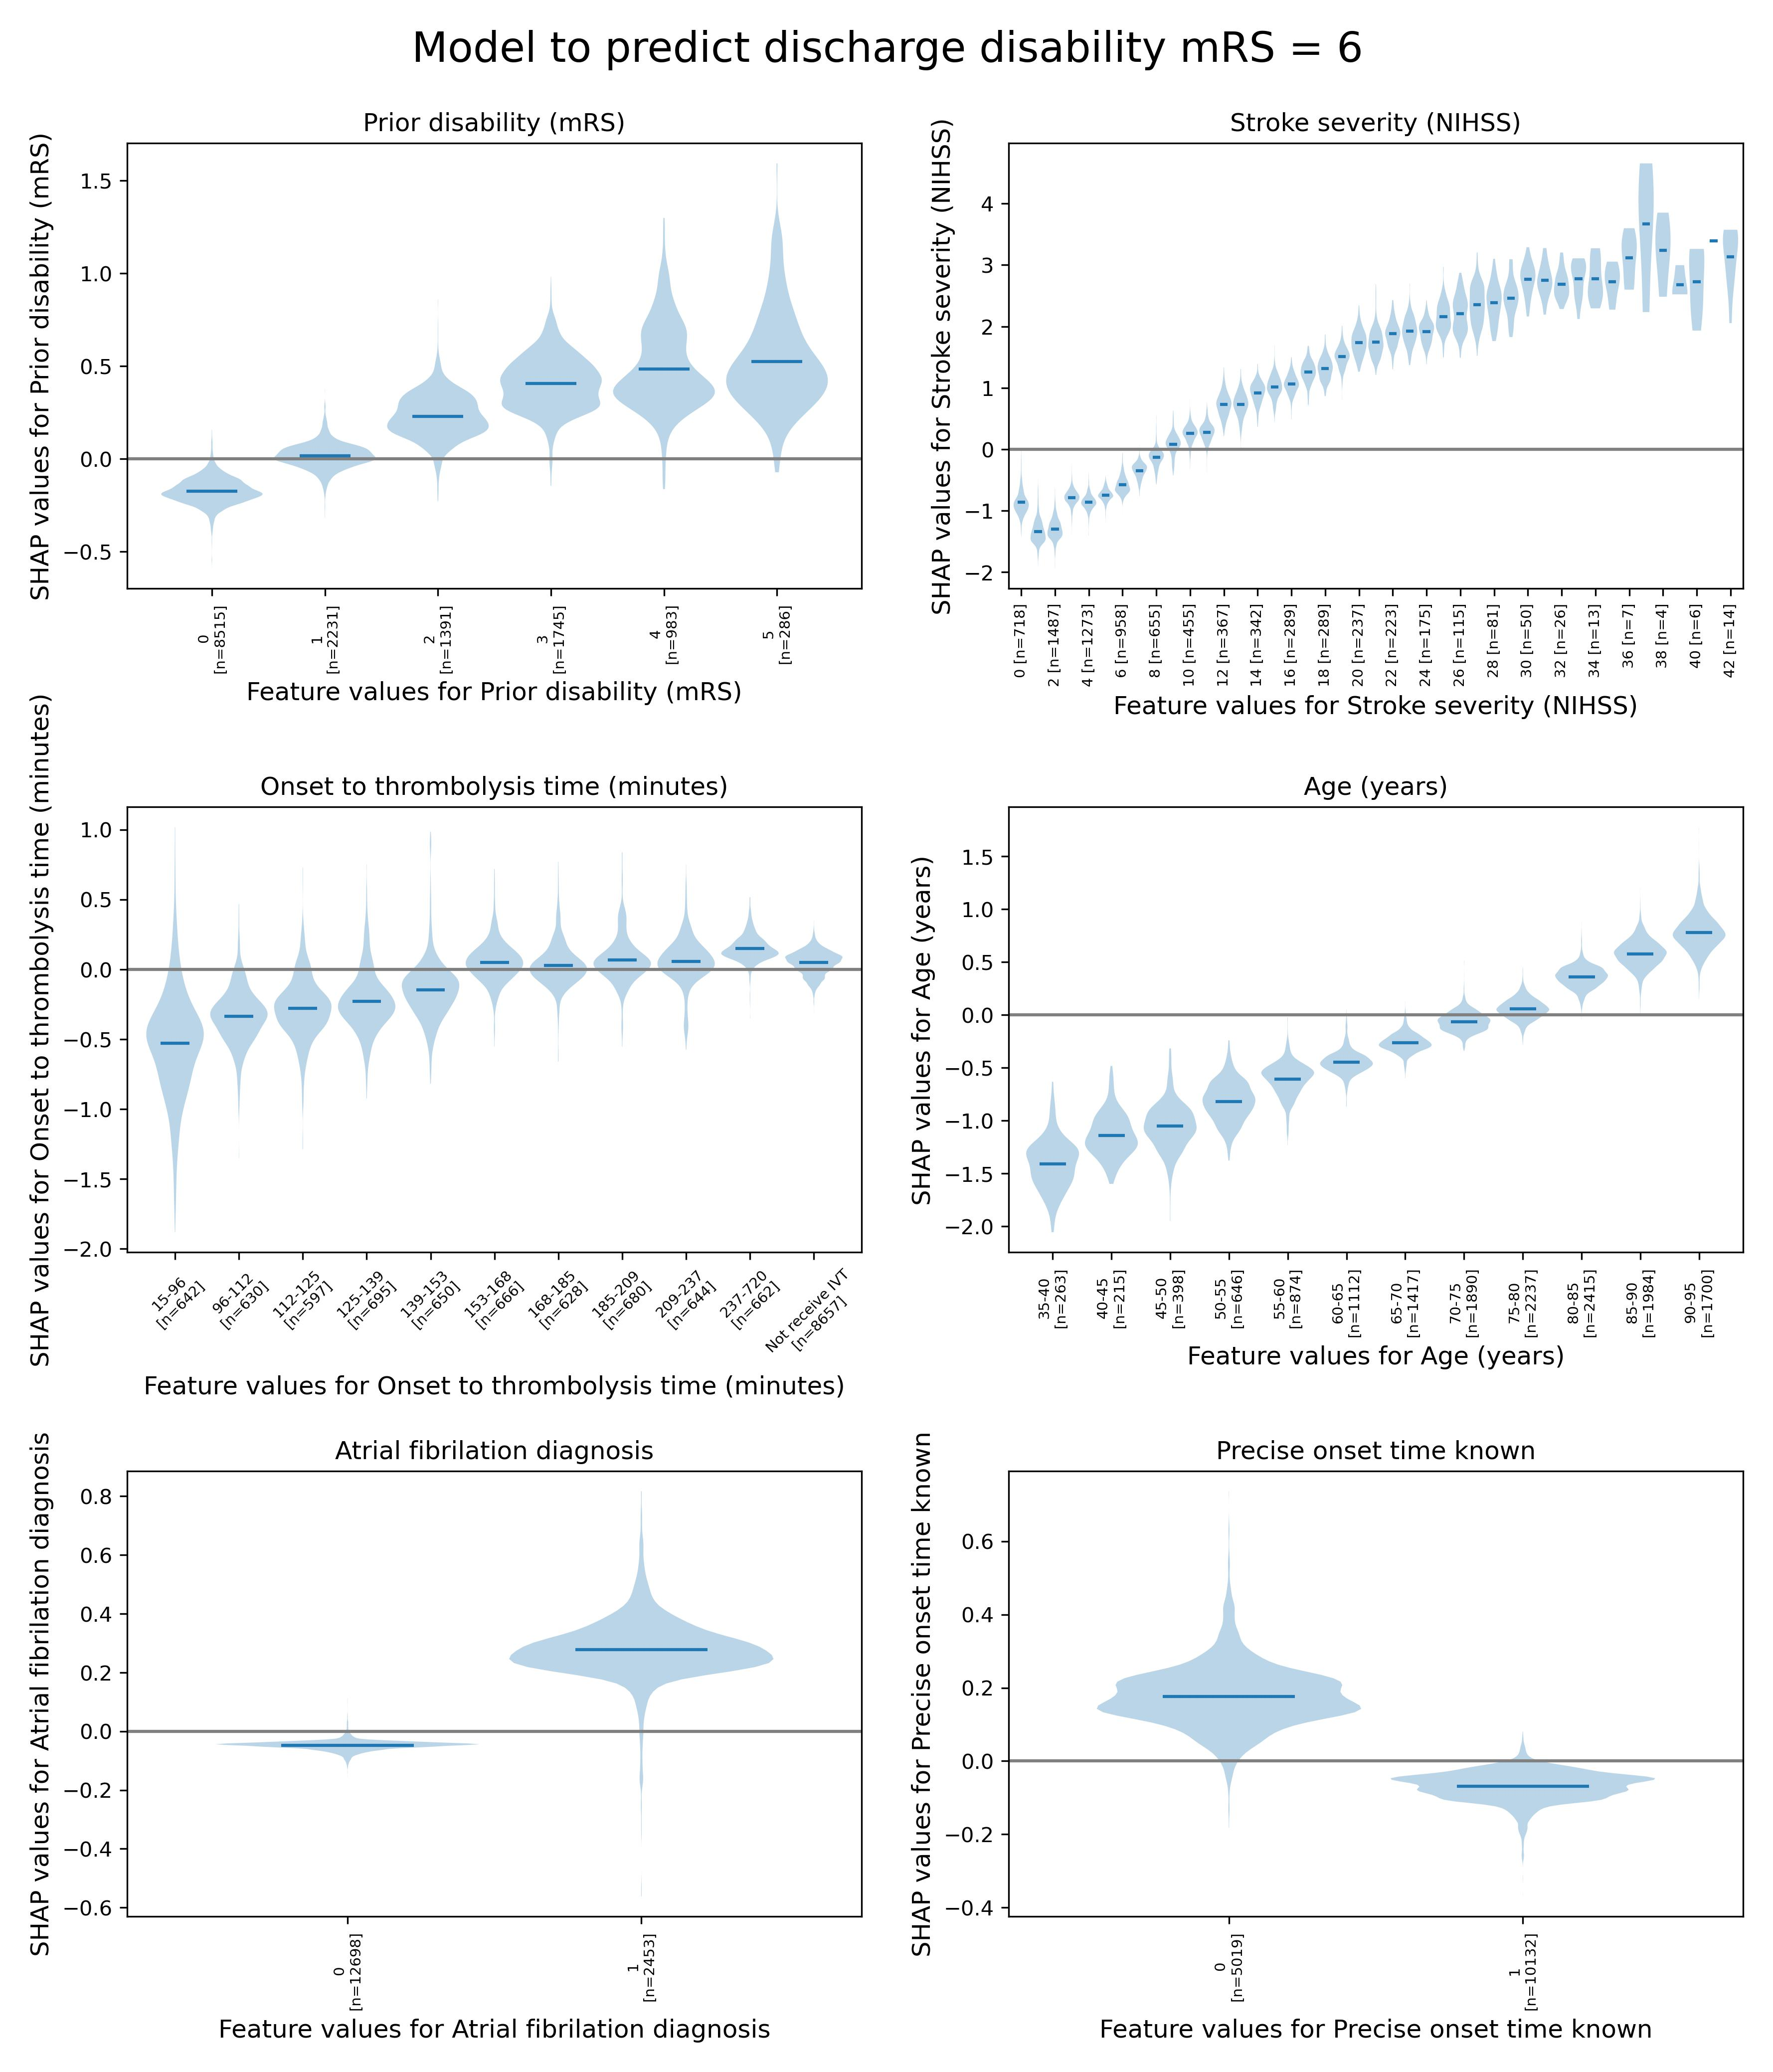
\includegraphics[trim={0 0 0 1.2cm}, clip, width=0.95\linewidth]      {./images/053_xgb_7_features_1fold_thrombolysis_shap_violin_all_features_for_mRS6}\\%{./images/053_predict_mrs6_split_by_ss.png}\\
      %{./images/053_xgb_7_features_1fold_999999_thrombolysis_shap_violin_all_features_for_mRS6}\\%{./images/053_predict_mrs6_split_by_ss.png}\\
%        \caption{Predict the likelihood of death on discharge (mRS 6)}
%        \label{fig:mrs6_violin_split}
    \end{subfigure}
    \hfill
    \begin{subfigure}{.5\textwidth}
      \centering
      \captionsetup{width=.9\linewidth}
      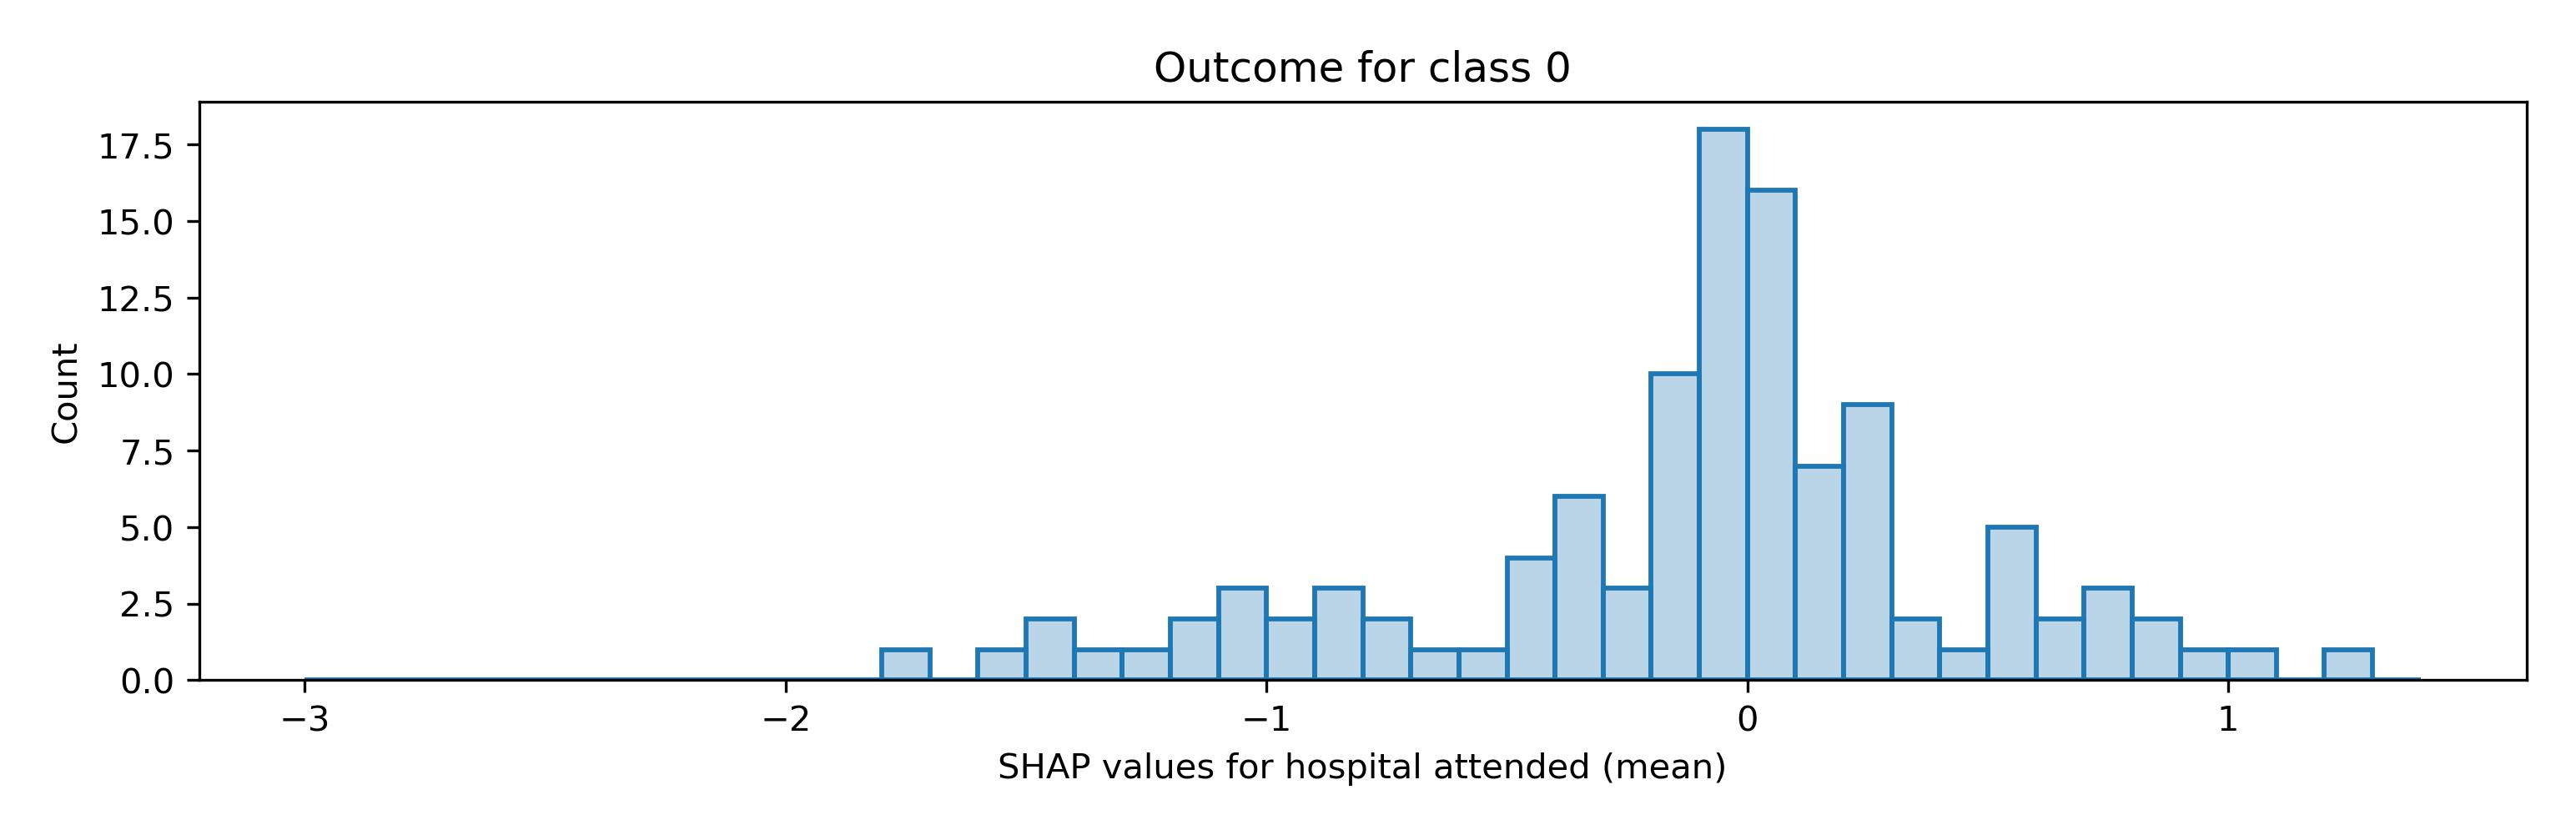
\includegraphics[trim={0 0 0 1cm}, clip, width=1\linewidth]    {./images/053_xgb_7_features_1fold_hosp_shap_hist_mrs0}\\%{./images/053_xgb_7_features_1fold_999999_hosp_shap_hist_mrs0}\\
      \caption{\footnotesize{SHAP values for the likelihood of no disability on discharge (mRS 0). Base SHAP value = -0.405}}
      \label{fig:mrs0_violin}
    \end{subfigure}%ults
    \begin{subfigure}{.5\textwidth}
      \centering
      \captionsetup{width=.9\linewidth}
      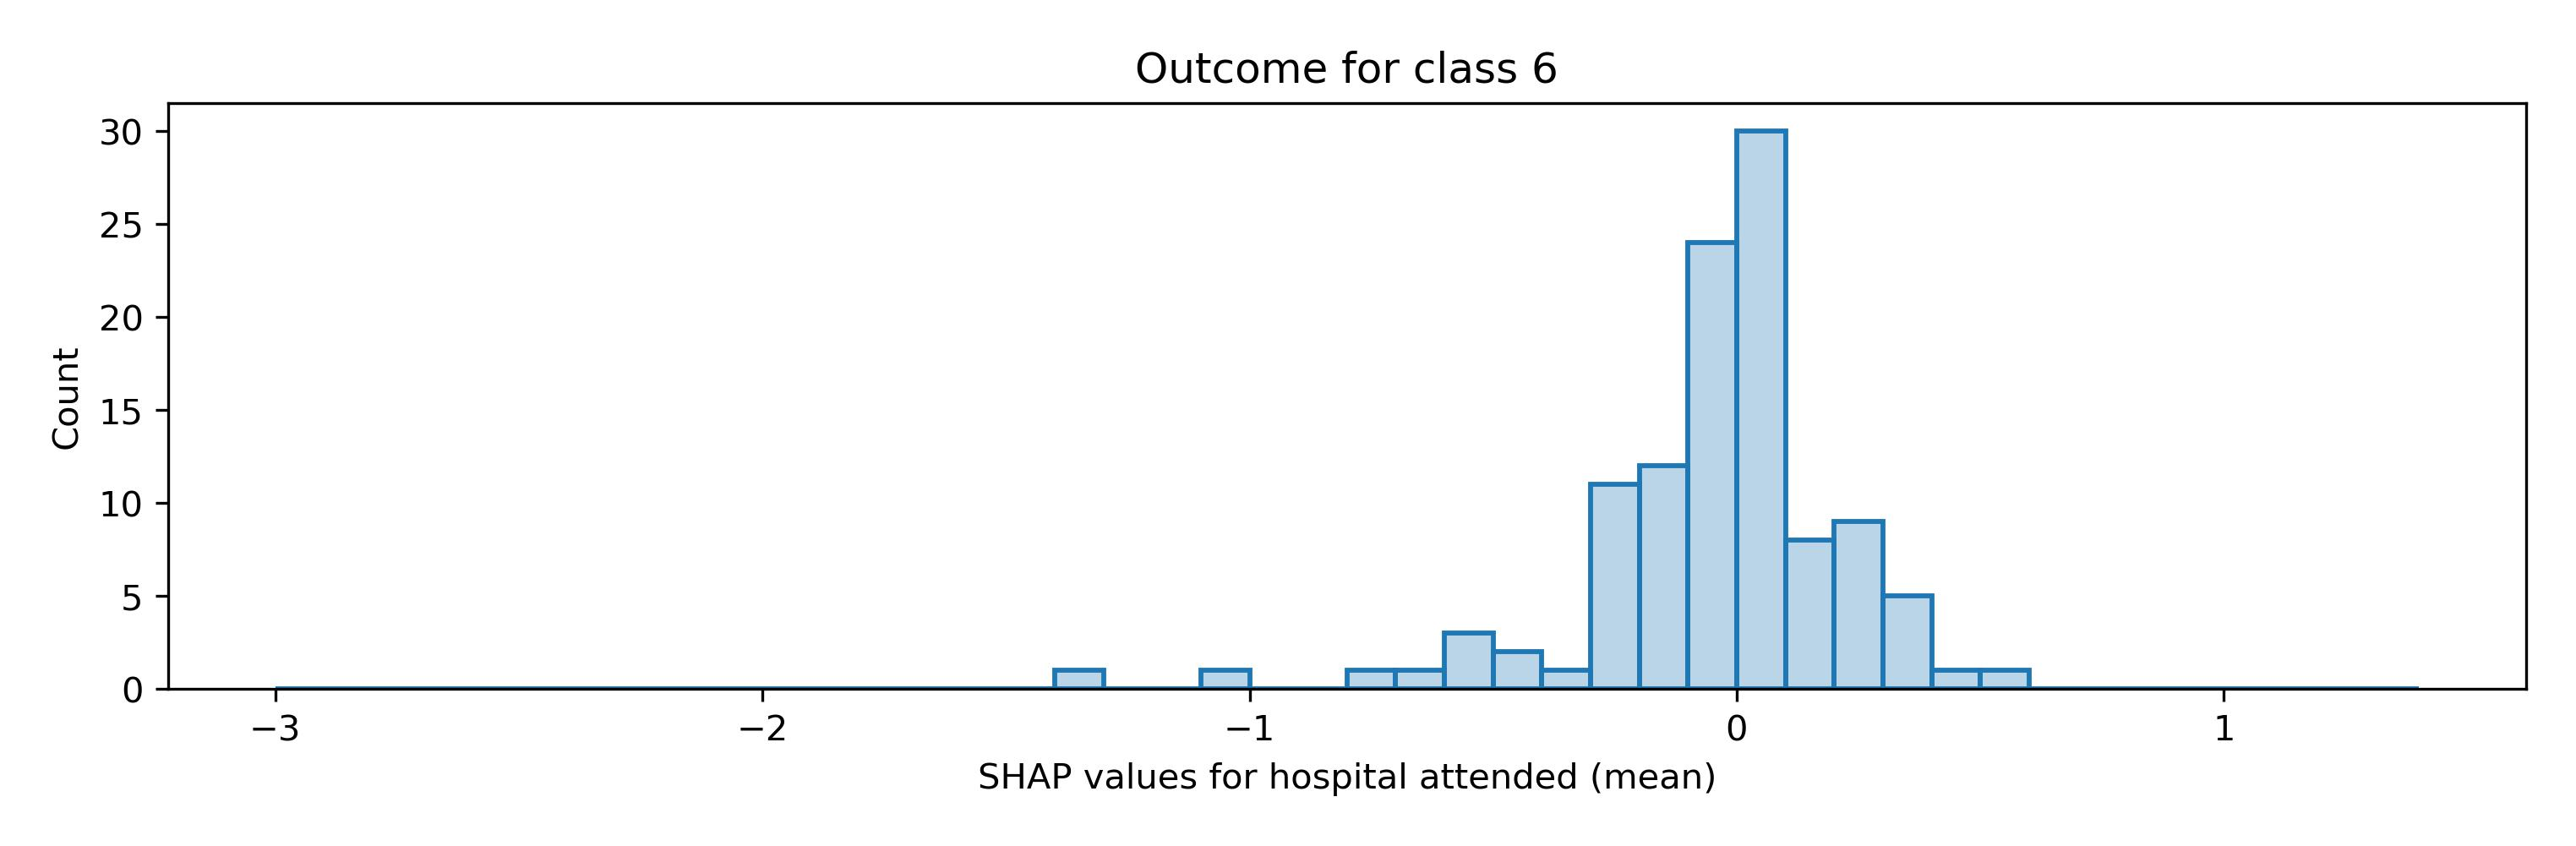
\includegraphics[trim={0 0 0 1cm}, clip, width=1\linewidth]
        {./images/053_xgb_7_features_1fold_hosp_shap_hist_mrs6}\\
%        {./images/053_xgb_7_features_1fold_999999_hosp_shap_hist_mrs6}\\
      \caption{\footnotesize{SHAP values for the likelihood of death at discharge (mRS 6). Base SHAP value = -0.311}}
      \label{fig:mrs6_violin}
    \end{subfigure}
  \caption{Plots showing the relationship between SHAP values and feature values for best or worse possible outcomes. Left: Predicting the likelihood of having no disability at discharge (mRS 0). Right: Predicting the likelihood of being dead at discharge (mRS 6). Top: Violin plots showing the relationship between SHAP values and feature values. The horizontal line shows the median SHAP value. Bottom: Histogram showing the frequency of the mean SHAP value for the hospital attended.}
    \label{fig:shap_outcome_model}
\end{figure}

%%%%%%%%%%%%%%%%%%%%%% PROTOTYPE PATIENTS %%%%%%%%%%%%%%%%%%%%%%%%%%%%


\subsection{Prototype patients and the effect of thrombolysis on outcomes}

In order to further understand and illustrate the effect of thrombolysis on outcomes we created eight \textit{prototype} patients. The base patient in these patients was a patient that would generally be considered an ideal candidate for thrombolysis. We then altered each feature of that patient in a controlled way. This gave the following patients:

\begin{enumerate}
    \item \textit{Ideal}: No prior disability (mRS 0), age 72.5, no atrial fibrillation diagnosis, NIHSS 15, precise onset time, onset to thrombolysis time 2 hours. The patient attended a hospital with the most neutral contribution towards use of thrombolysis.
    \item \textit{Mild stroke}: As \textit{Ideal} but NIHSS 3
    \item \textit{Severe stroke}: As \textit{Ideal} but NIHSS 25
    \item \textit{Prior disability 3}: As \textit{Ideal} but prior disability mRS 3
    \item \textit{Prior disability 4}:  As \textit{Ideal} but prior disability mRS 4
    \item \textit{Atrial fibrillation diagnosis}: As \textit{Ideal} but with an atrial fibrillation diagnosis
    \item \textit{Older}: As \textit{Ideal} but age 87.5
    \item \textit{Imprecise onset time}: As \textit{Ideal} but imprecise onset time
\end{enumerate}

We predicted mRS distributions for each patient with and without thrombolysis. We also classified whether the patient would likely have both an improvement in the probability-weighted disability at discharge and a reduction in probability of having the worst outcomes of mRS 5-6. Results are shown in figure \ref{fig:counterfactual_bar_plot}. Thrombolysis was predicted to improve outcomes across all patients, but the benefit was significantly lower with mild stroke.

\begin{figure}
\centering
 {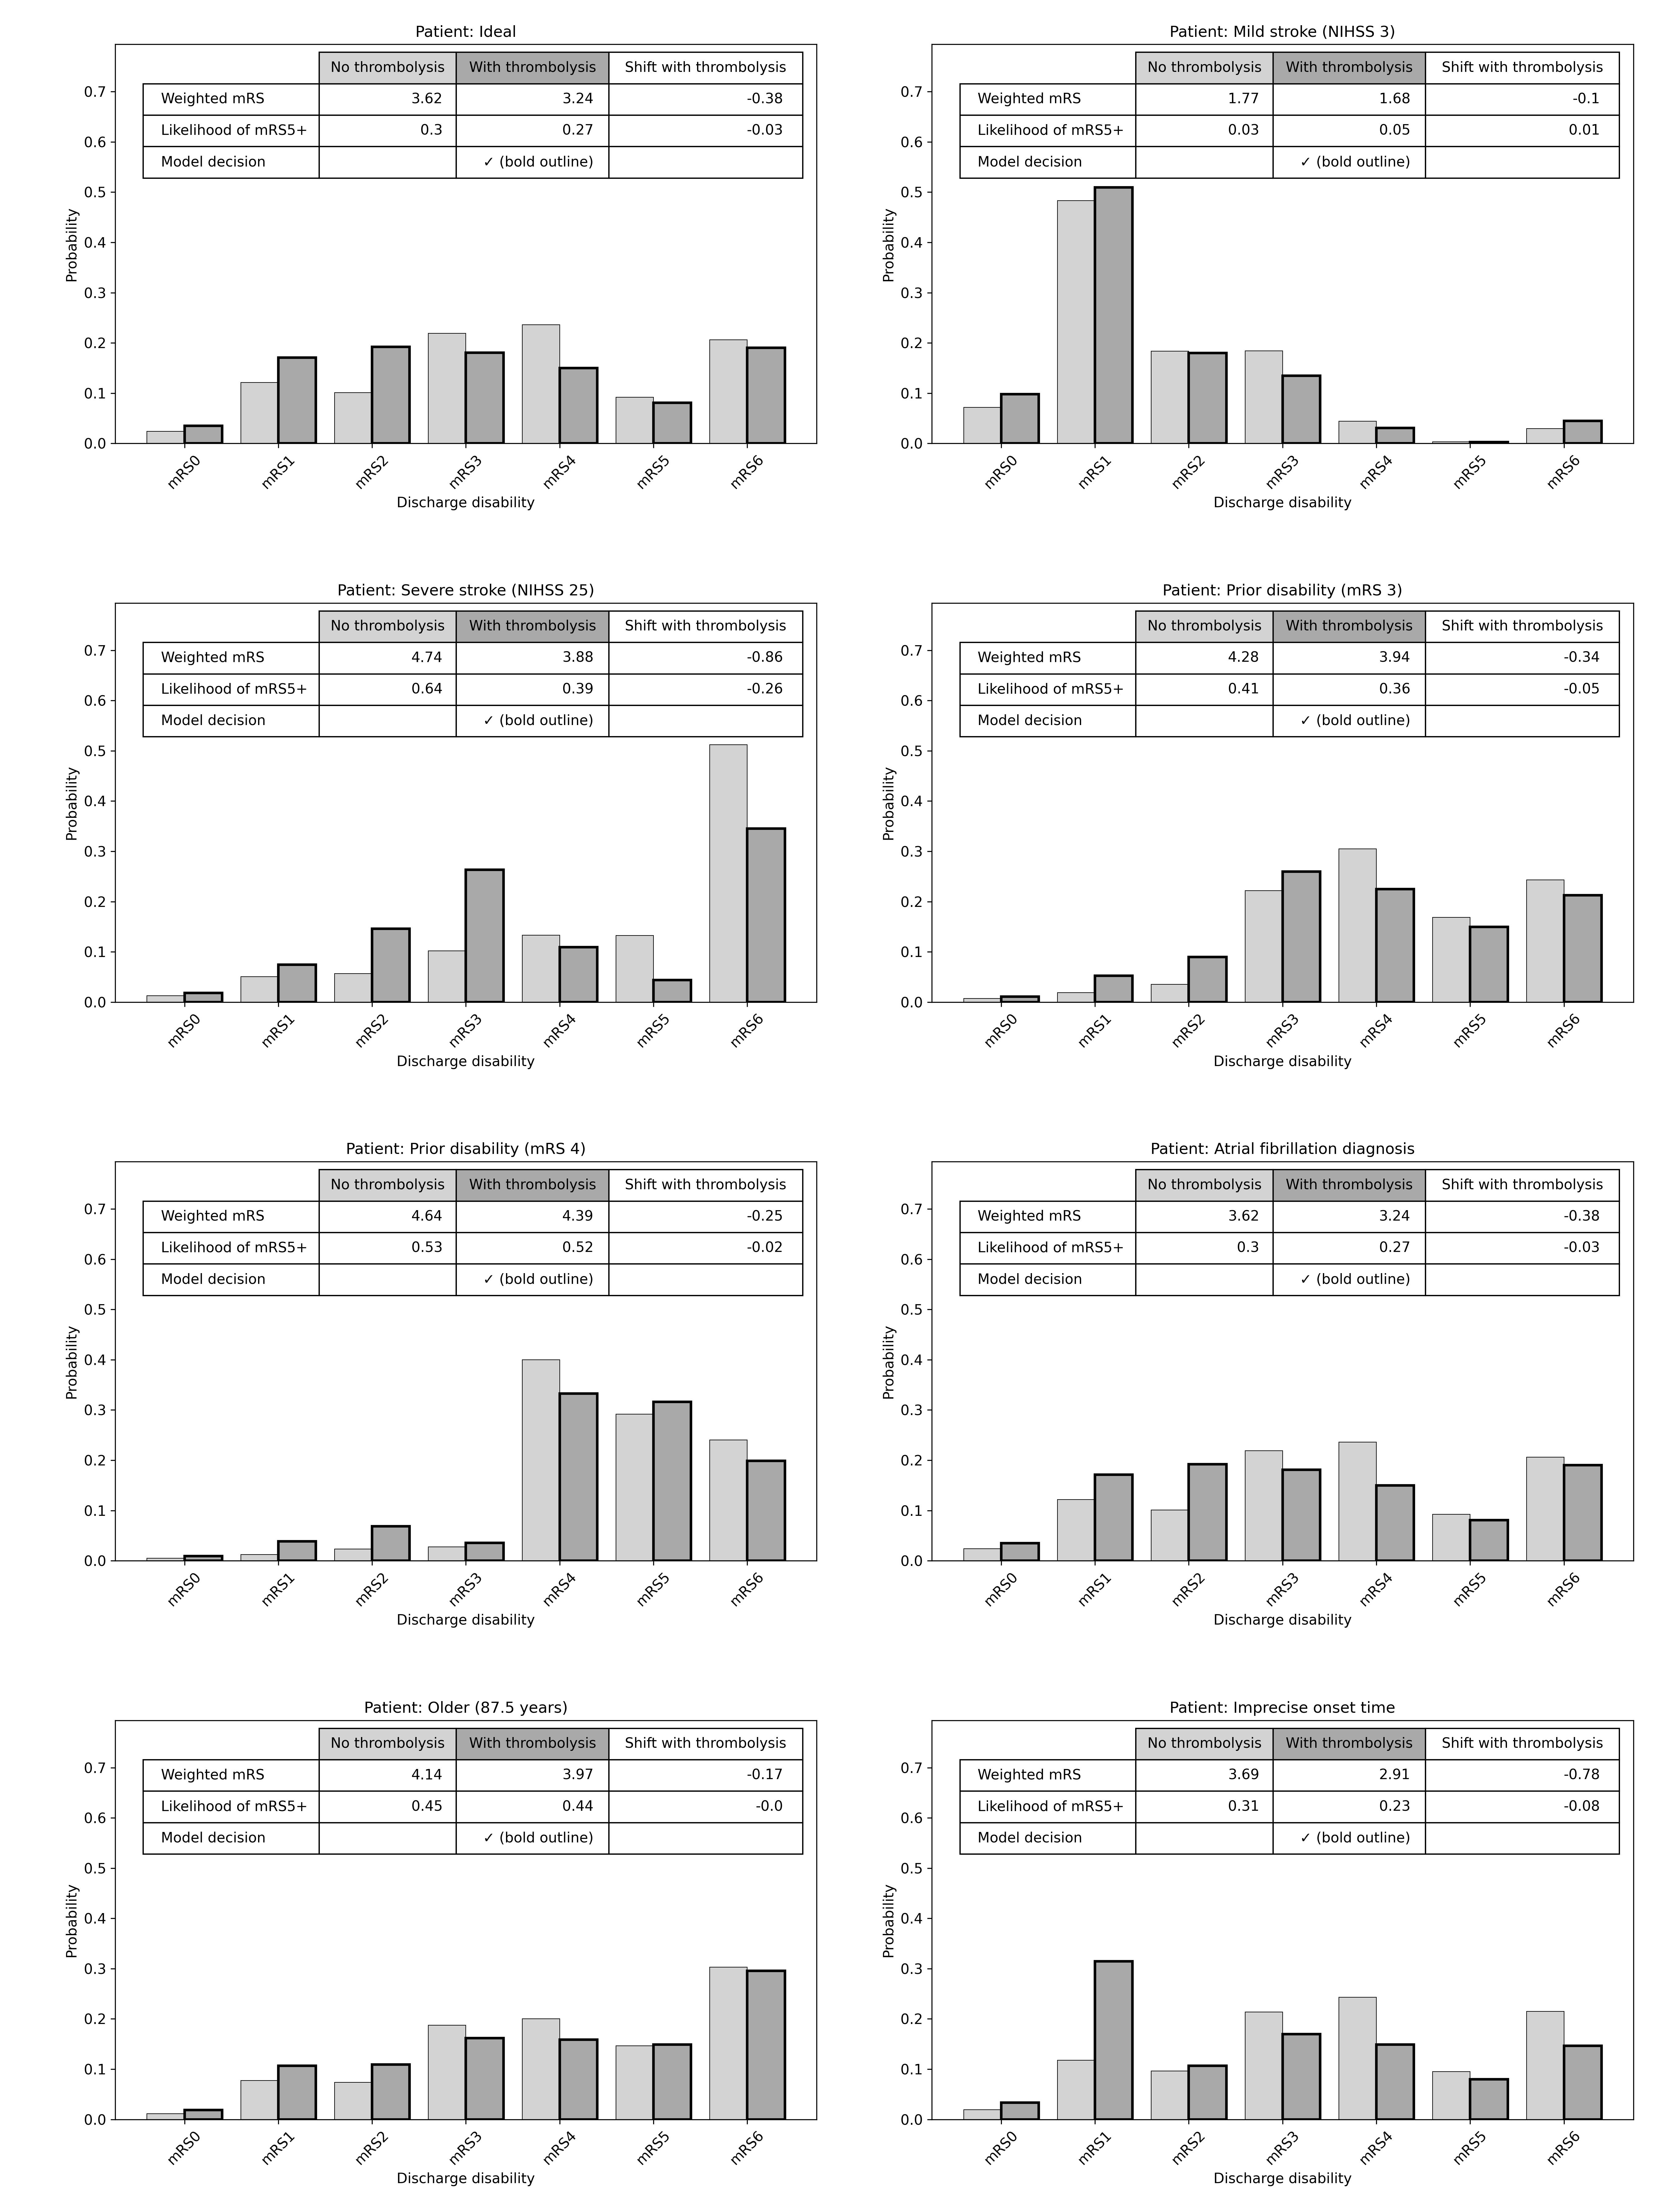
\includegraphics[width = 6.1in]{./images/060_xgb_mrs_distributions_bar_plot_table_bw.jpg}}\\%{./images/060_xgb_mrs_distributions_999999_bar_plot.jpg}}\\%060_bar_plot.png}}\\
 \caption{Probability distribution of disability at discharge (as mRS score) for eight defined patients. i. \textit{Ideal}: No prior disability (mRS 0), age 72.5, no afib diagnosis, NIHSS 15, precise onset time, onset to treatment 2 hours, attended stroke team with most neutral contribution towards use of thrombolysis. ii. \textit{Mild stroke}: As \textit{Ideal} but NIHSS 3. iii. \textit{Severe stroke}: As \textit{Ideal} but NIHSS 25. iv. \textit{Prior disability (mRS3)}: As \textit{Ideal} but prior disability mRS 3. v. \textit{Prior disability (mRS 4)}:  As \textit{Ideal} but prior disability mRS 4. vi. \textit{Atrial fibrillation diagnosis}: As \textit{Ideal} but with an atrial fibrillation diagnosis. vii. \textit{Older (87.5 years)}: As \textit{Ideal} but age 87.5. viii. \textit{Imprecise onset time}: As \textit{Ideal} but imprecise onset time. Inset table shows the values for the two criteria that defines whether a patient has a better outcome with thrombolysis, and the treatment decision that this method would decide.}
 \label{fig:counterfactual_bar_plot}
\end{figure}

%%%%%%%%%%%%%%%%%%%%%% SCATTER PLOT %%%%%%%%%%%%%%%%%%%%%%%%%%%%

\subsection{Comparing actual use of thrombolysis and predicted benefit from thrombolysis}

In the first k-fold test set of 15,680 patients, 44\% received thrombolysis. For each patient we predicted outcomes with and without thrombolysis. Figure \ref{fig:scatter_all} shows the expected shift in probability-weighted mRS at discharge, and the change in probability of being discharged with mRS 5-6, due to thrombolysis, separated by whether the patient actually received thrombolysis or not. Overall, 60\% of patients were predicted to benefit from thrombolysis. Of those who did receive thrombolysis, 73\% were predicted to have both a better average disability likelihood and a reduction in probability of being mRS 5-6. 9\% were predicted to have both a worse average disability likelihood and an increase in probability of being mRS 5-6. 18\% were predicted to have either, but not both, an improved average disability likelihood or a reduction in probability of being mRS 5-6. Of those who did not receive thrombolysis, 49\% were predicted to have both a better average disability likelihood and a reduction in probability of being mRS 5-6. 26\% were predicted to have both a worse average disability likelihood and an increase in probability of being mRS 5-6. 25\% were predicted to have either, but not both, an improved average disability likelihood or a reduction in probability of being mRS 5-6.

\begin{figure}
\centering
\begin{subfigure}{.7\textwidth}
  \centering
  \captionsetup{width=.9\linewidth}
  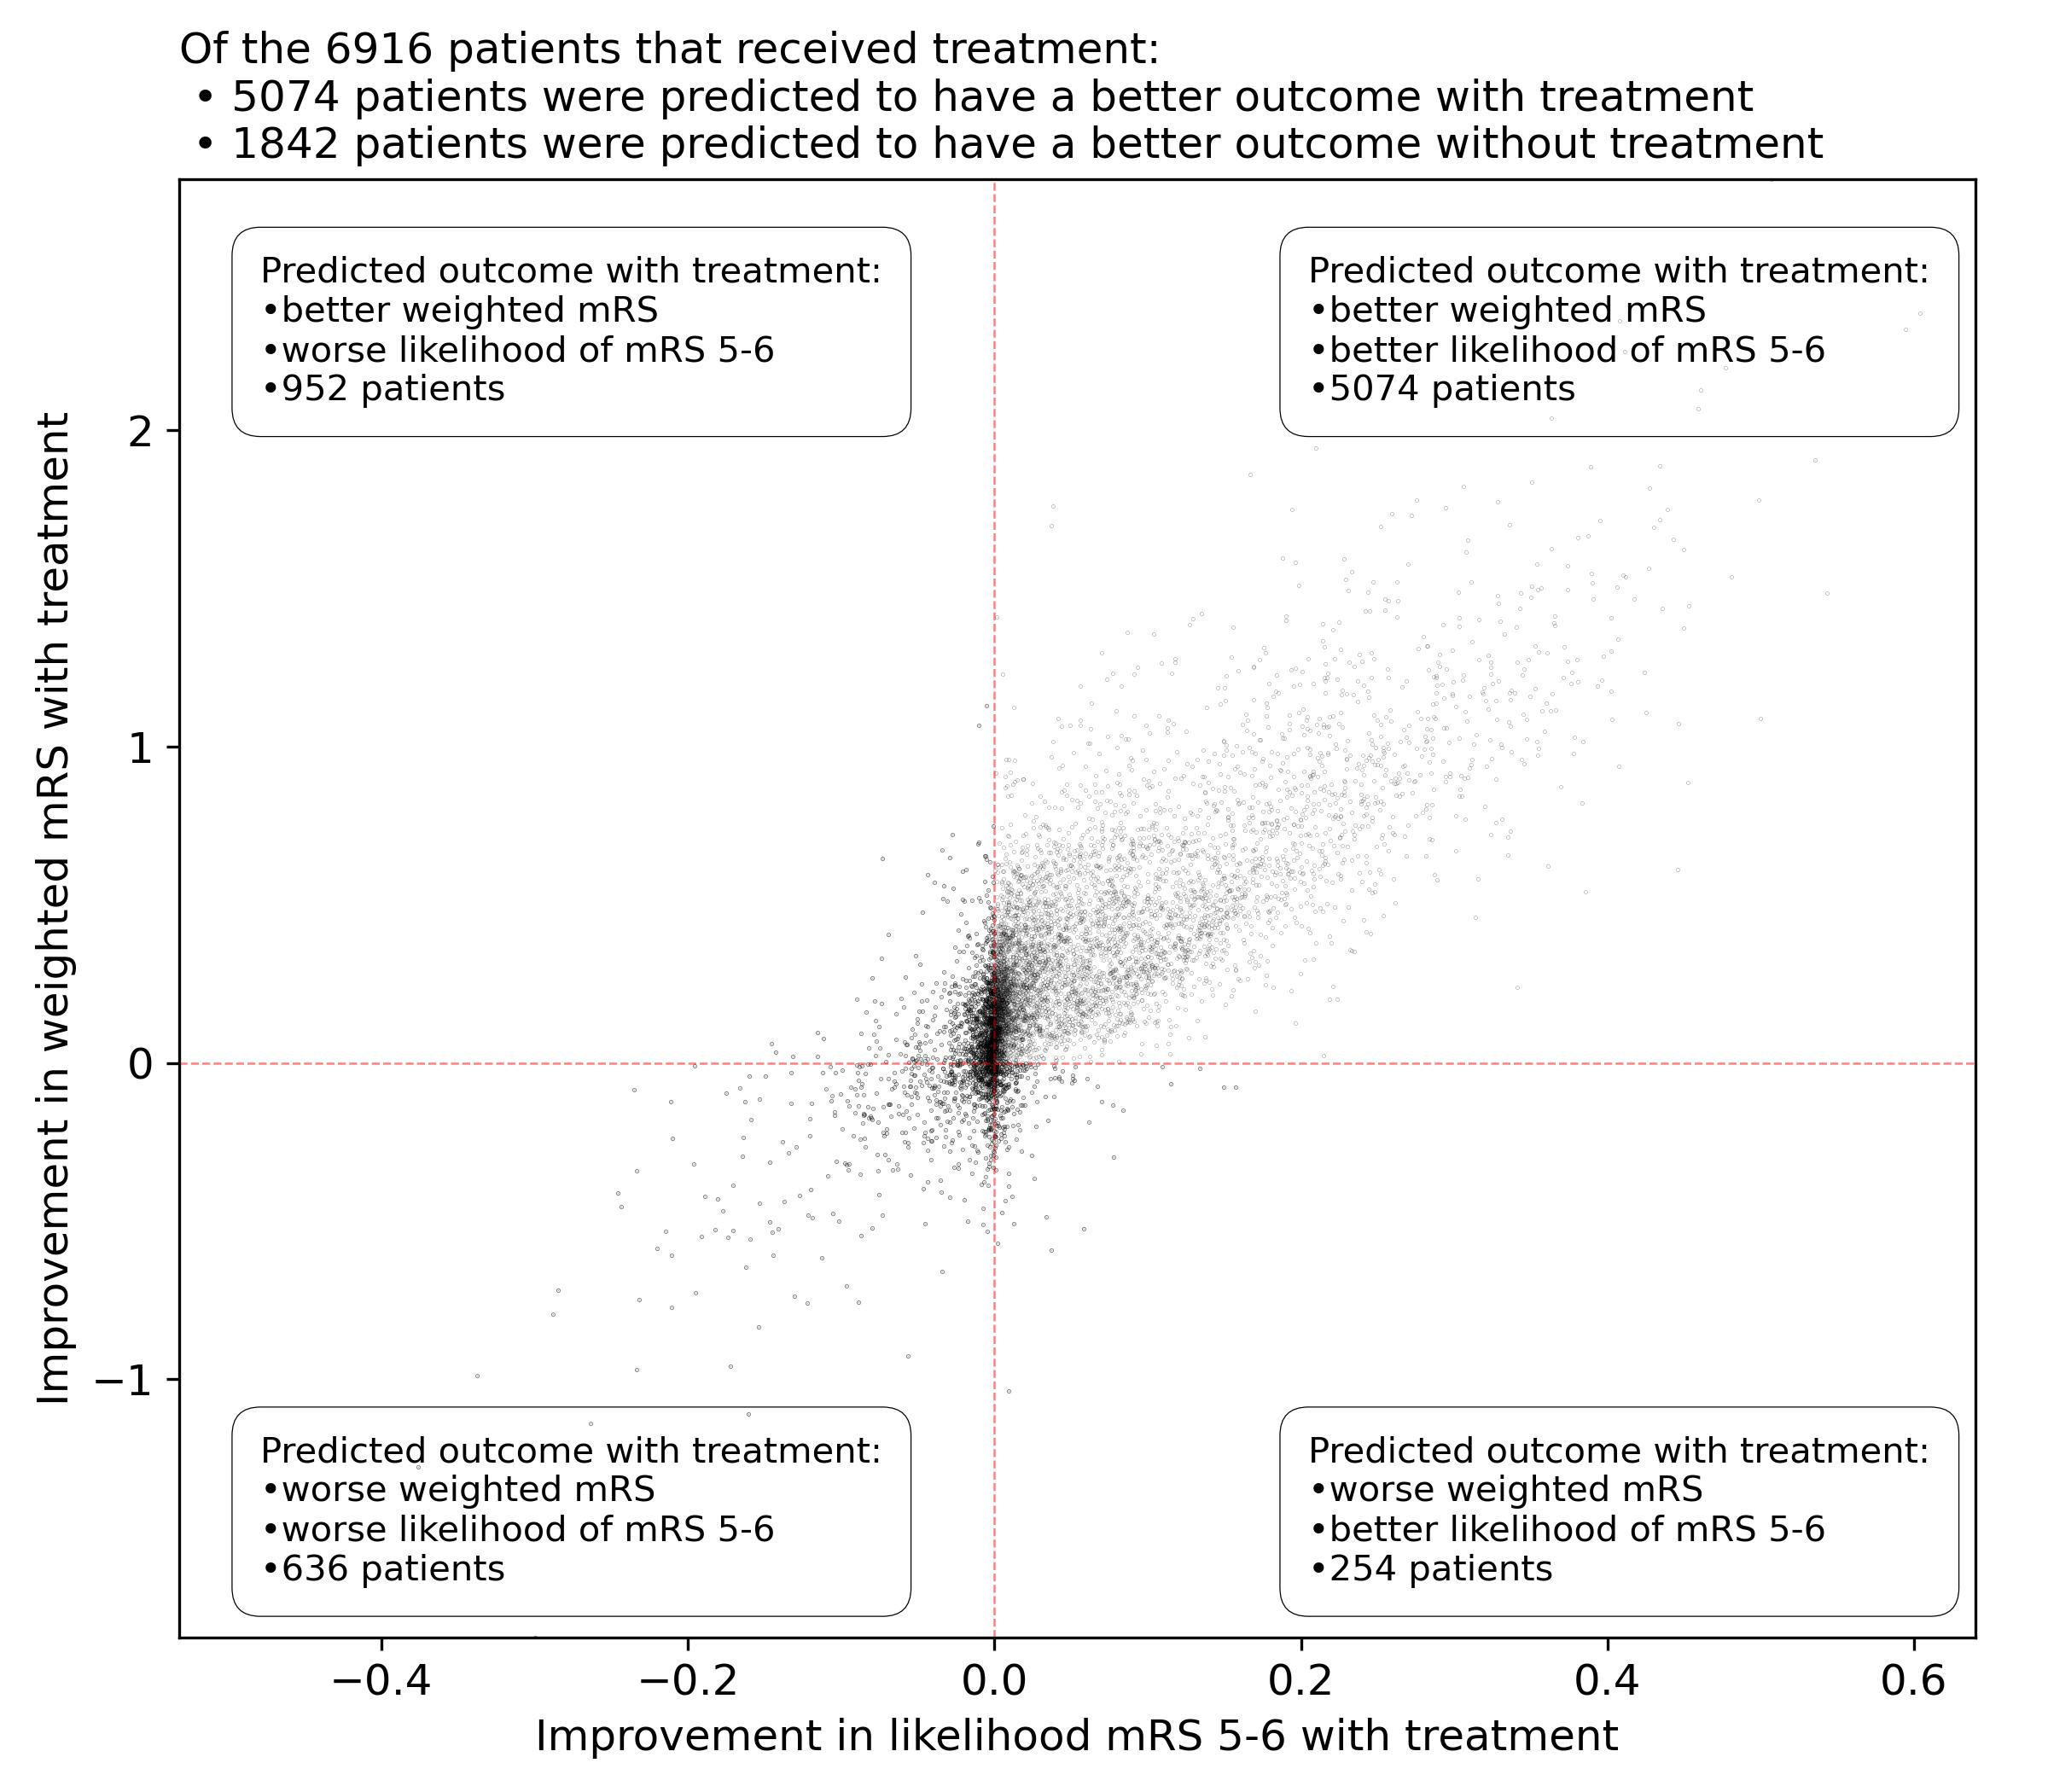
\includegraphics[trim={0 0 0 1.7cm}, clip, width=1\linewidth]{./images/210_xgb_all_data_multiclass_outcome_scatter_criteria_treated}%210_better_outcome_criteria_scatter_treated.png}
  \caption{\footnotesize{Patients who received thrombolysis  (n = 6,916)}}
  \label{fig:scatter_receive}
\end{subfigure}

\vspace{5mm}

\begin{subfigure}{.7\textwidth}
  \centering
  \captionsetup{width=.9\linewidth}
  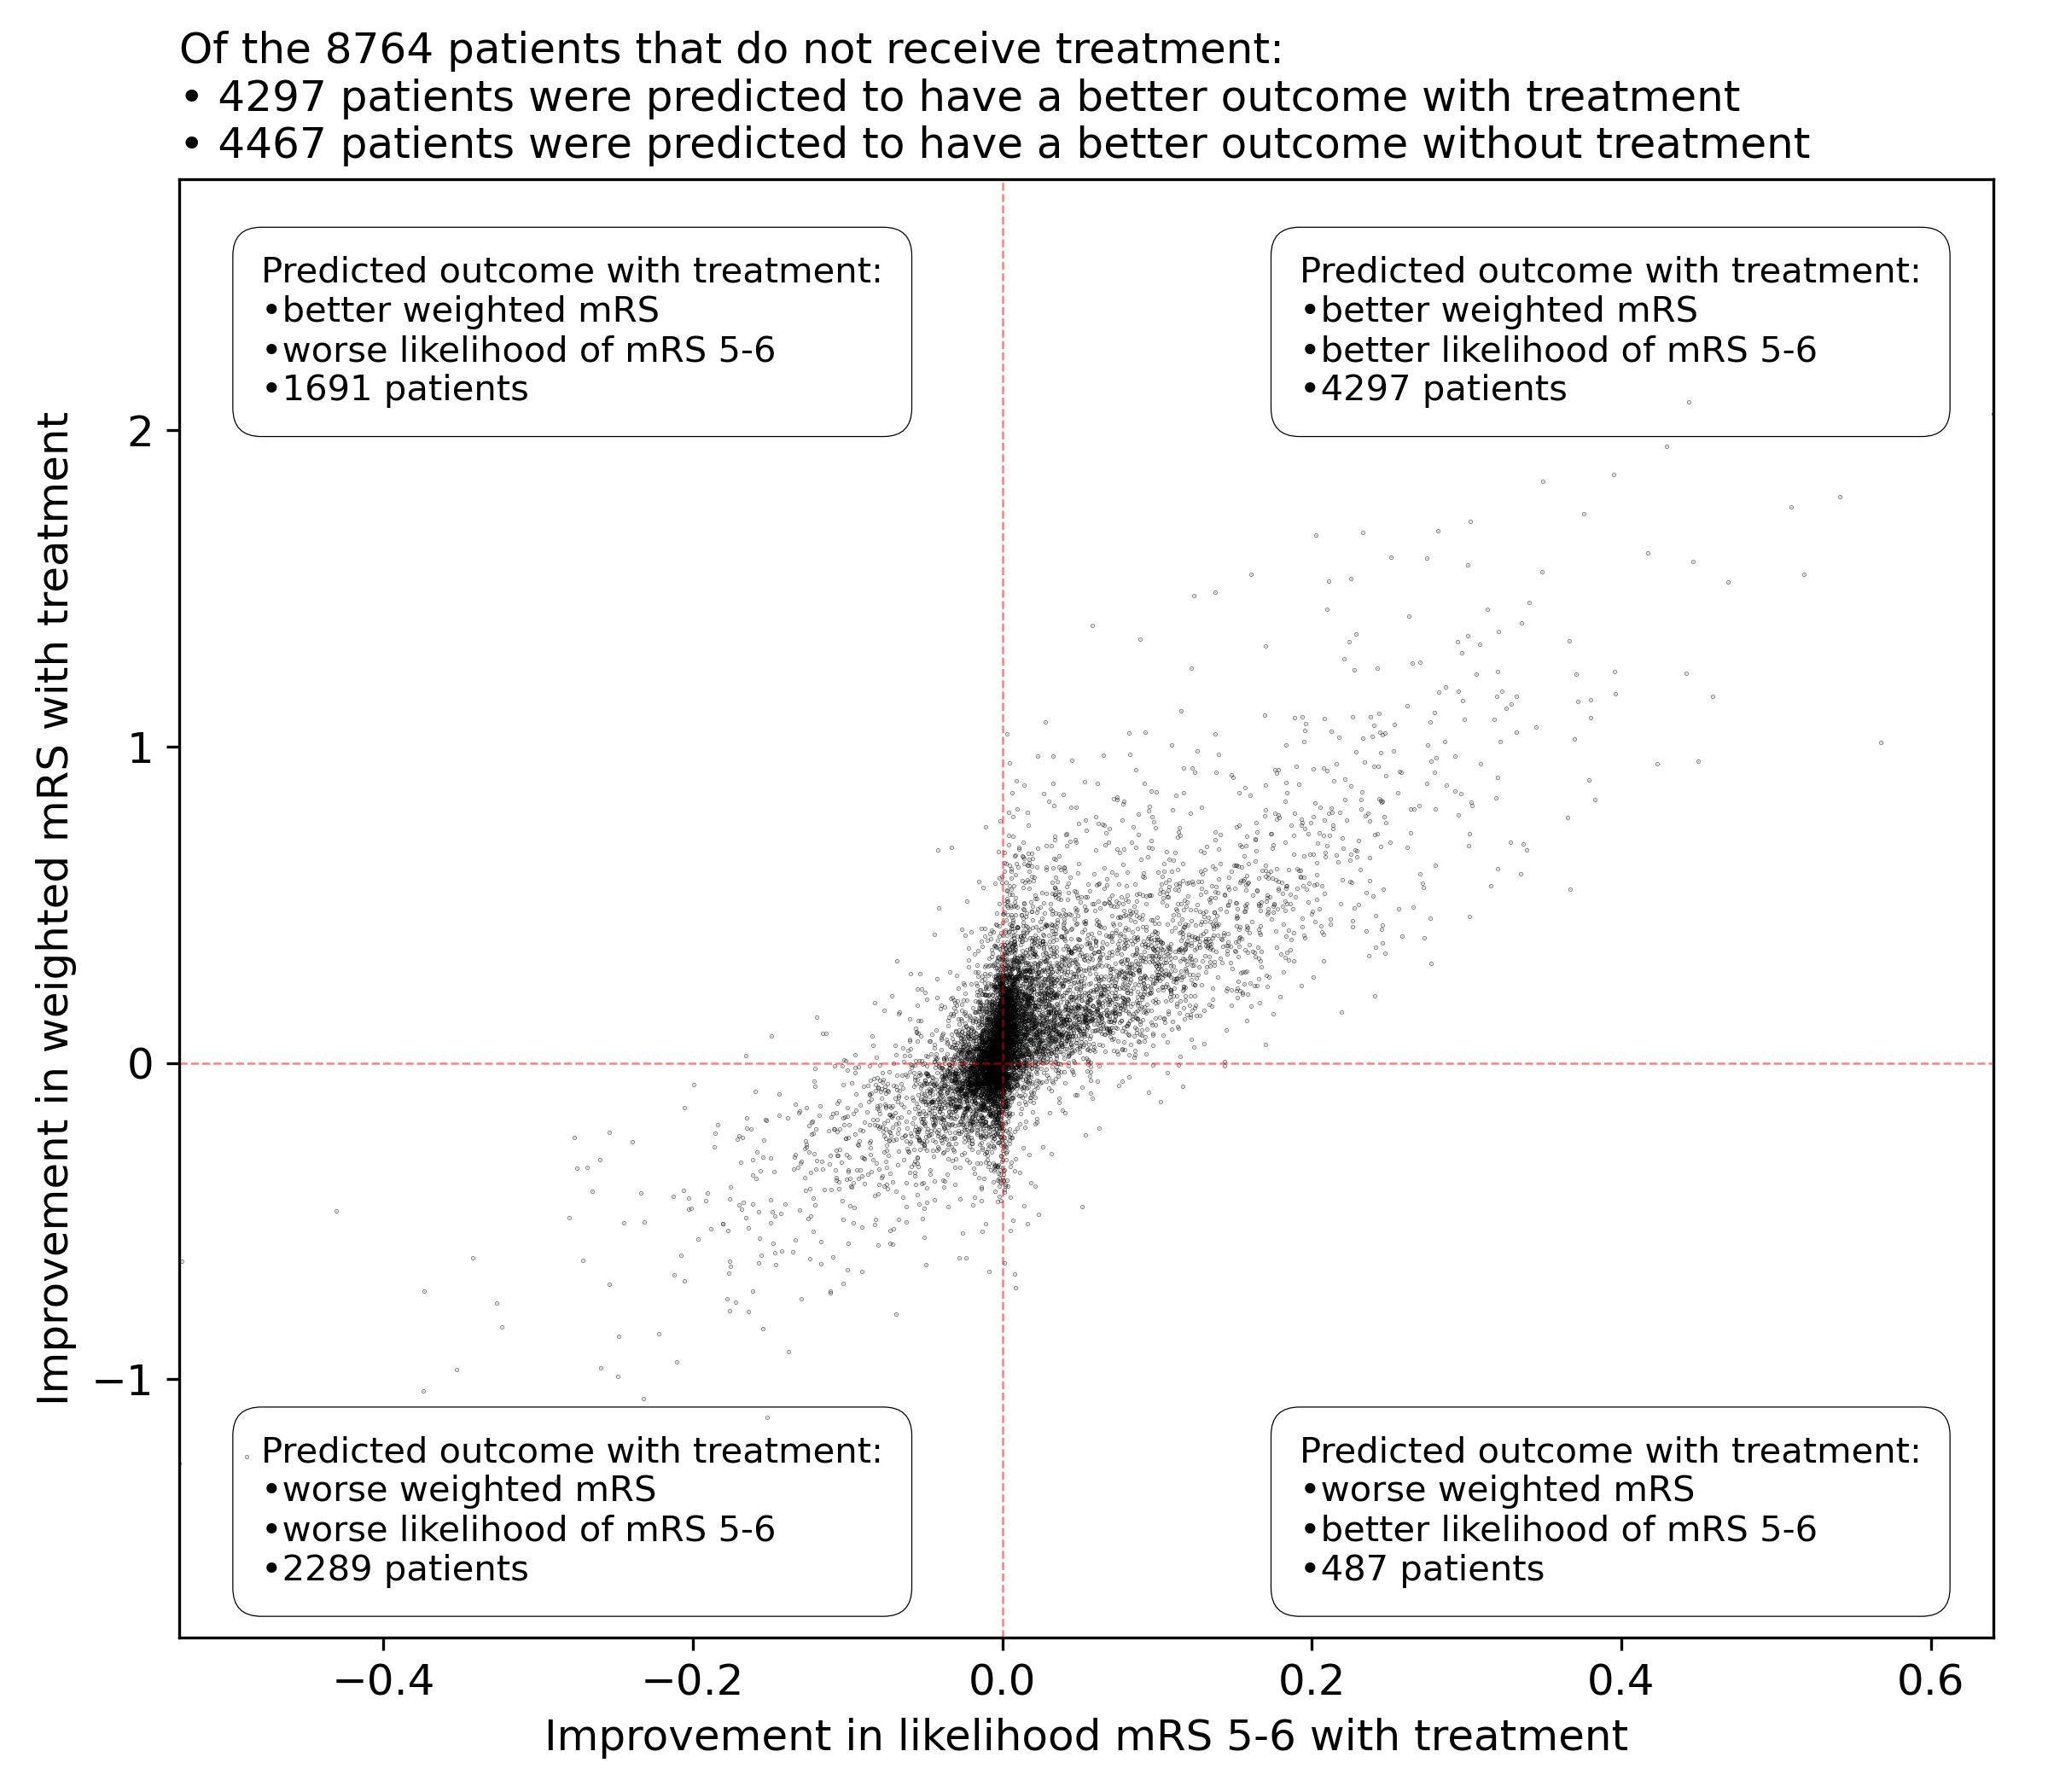
\includegraphics[trim={0 0 0 1.7cm}, clip, width=1\linewidth]{./images/210_xgb_all_data_multiclass_outcome_scatter_criteria_not_treated}%210_better_outcome_criteria_scatter_not_treated.png}
  \caption{\footnotesize{Patients who did not receive thrombolysis (n = 8,764)}}
  \label{fig:scatter_not_receive}
\end{subfigure}
  \caption{The predicted benefit or disbenefit of thrombolysis for each of 15,680 patients. Benefit is shown as both the expected improvement in probability-weighted disability (y-axis) and the improvement in likelihood of avoiding discharge with mRS 5-6. Both measures are expressed so that a positive value is better (a reduction in probability-weighted disability or a reduction in probability of discharge with mRS 5-6). (a) Patients who did actually receive thrombolysis (n = 6,916), (b) Patients who did not actually receive thrombolysis (n = 8,764).}
\label{fig:scatter_all}
\end{figure}

%%%%%%%%%%%%%%%%%%%%%% MISMATCH %%%%%%%%%%%%%%%%%%%%%%%%%%%%

\subsection{Patient characteristics that contribute to a mismatch between actual thrombolysis use and predicted best outcome}

Figure \ref{fig:decriptive_plots_2_cohorts} shows the distribution of feature values for two patient cohorts: (i) 1,842 patients that received thrombolysis but were predicted to not have a better outcome with thrombolysis, (ii) 4,297 that did not receive thrombolysis but were predicted to have a better outcome with thrombolysis.

When examining individual feature values in this way we did not identify any features that could be used in isolation to identify those patients who would benefit from thrombolysis but did not receive thrombolysis (or vice-versa). Patients who received thrombolysis but would likely not benefit from it have a range of feature values for each patient feature, as do those patients who did not receive thrombolysis but would benefit from it.

%./images/210_xgb_all_data_multiclass_outcome_999999_descriptive_plots_2_patient_cohorts
\begin{figure}
    \centering
    \captionsetup{width=1\linewidth}
    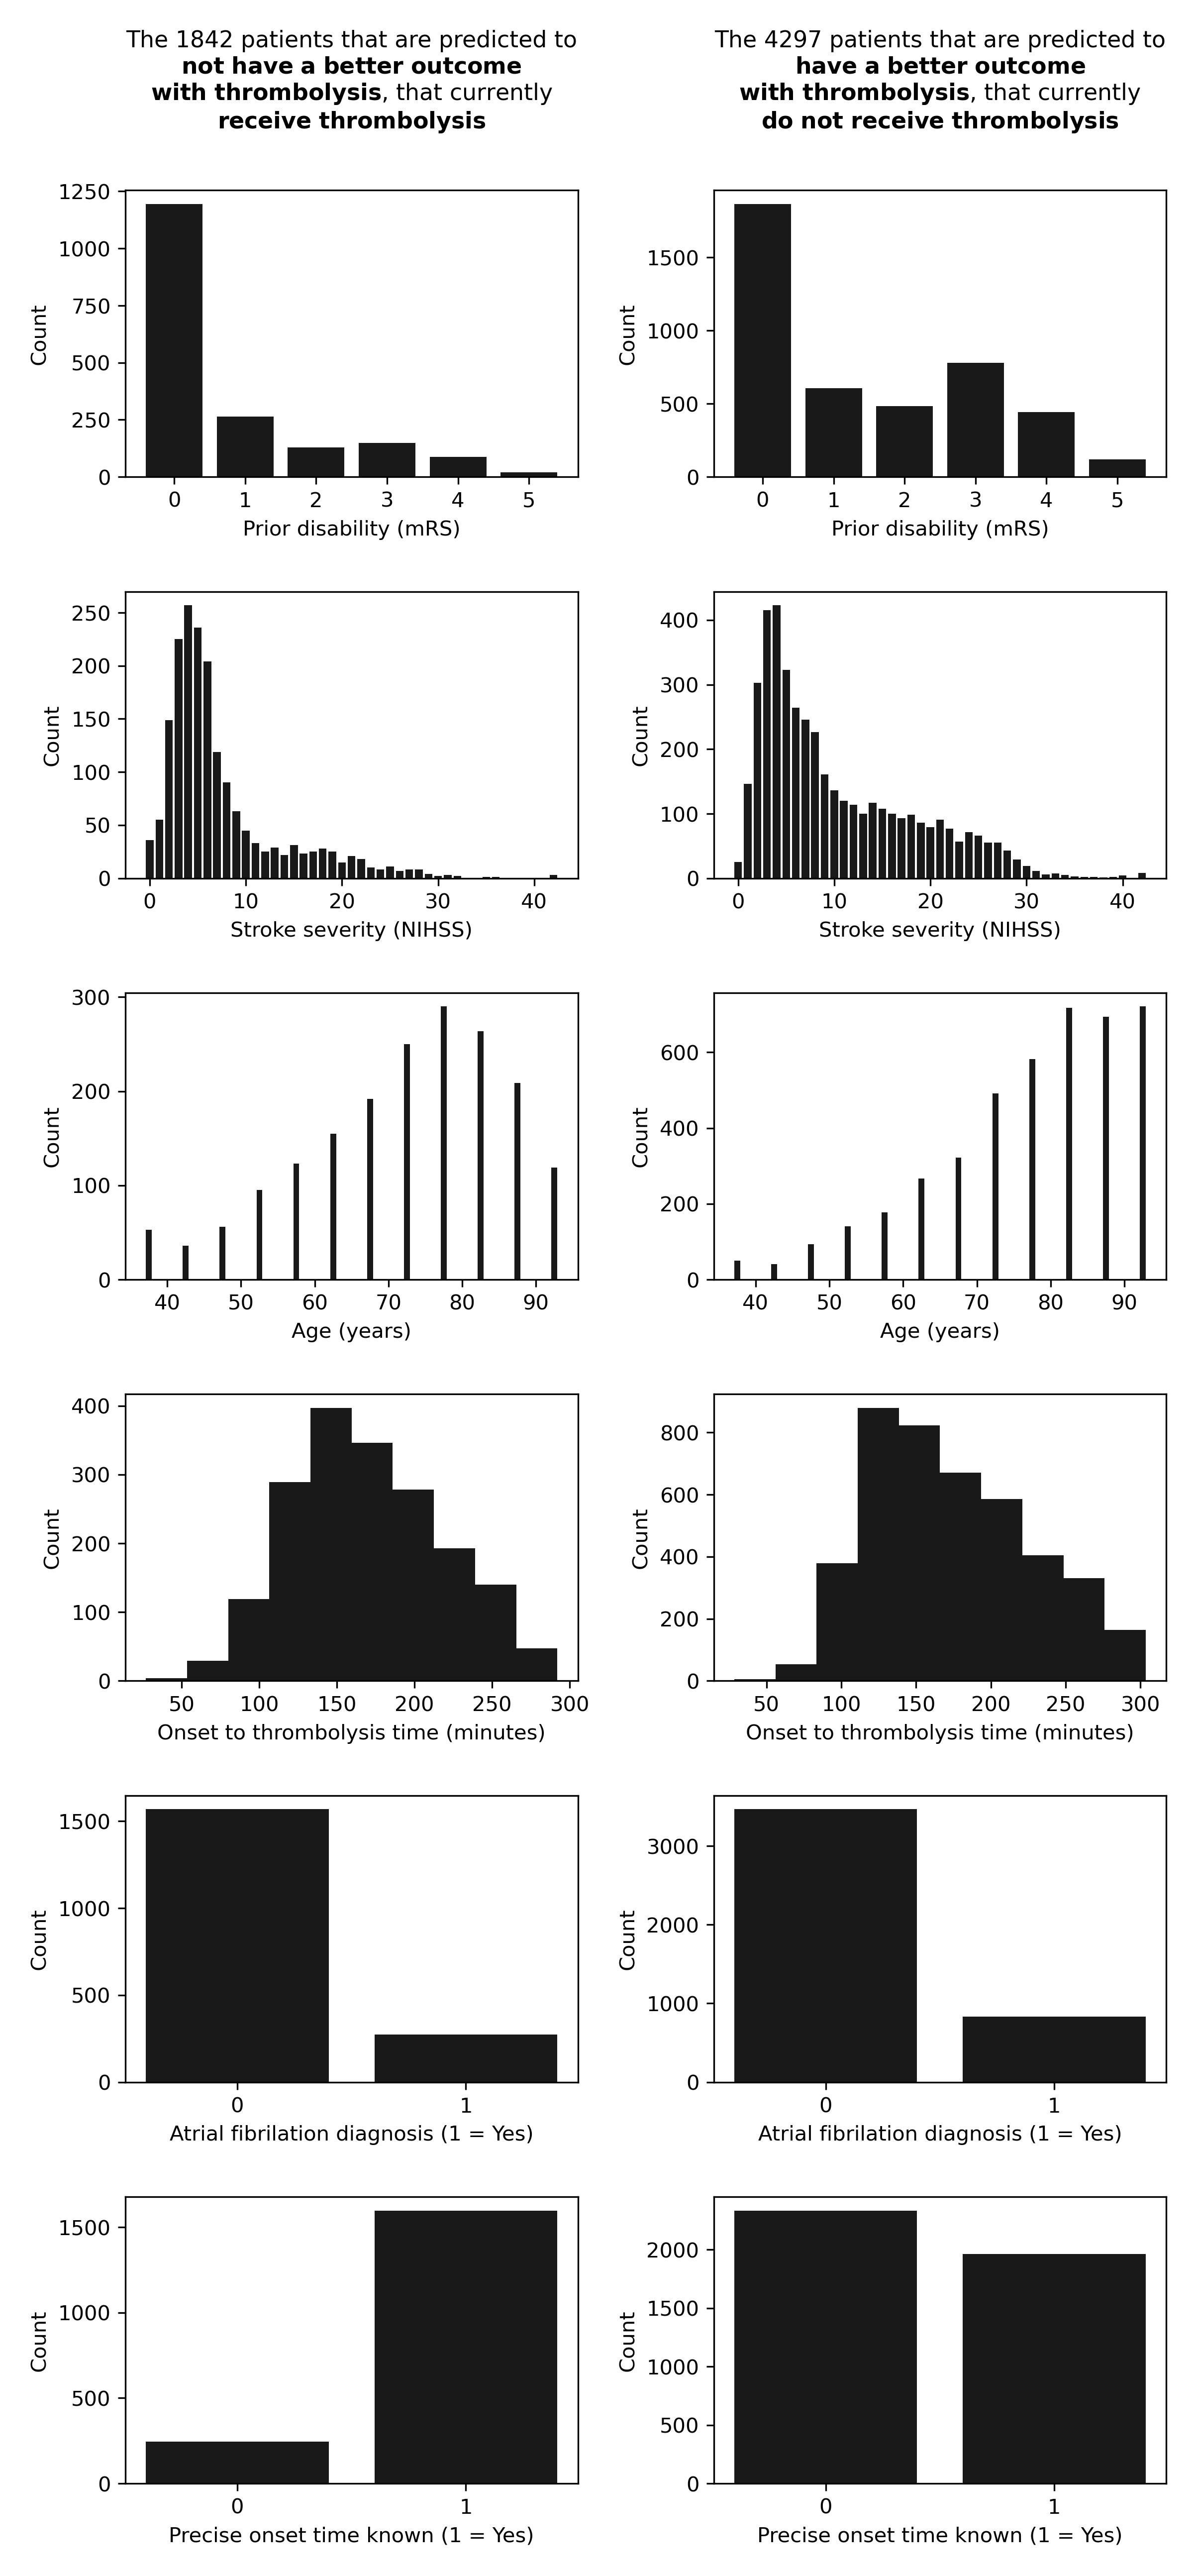
\includegraphics[width=0.6\linewidth]{./images/210_xgb_all_data_multiclass_outcome_descriptive_plots_2_patient_cohorts}\\
  \caption{Plots showing the frequency of feature values for patient cohorts where actual treatment decision differed from best predicted outcome. \textit{Left}: patients that were predicted to not have a better outcome with thrombolysis, but received thrombolysis. \textit{Right}: patients that were predicted to have a better outcome with thrombolysis, but did not receive thrombolysis.}
  \label{fig:decriptive_plots_2_cohorts}
\end{figure}

%%%%%%%%%%%%%%%%%%%%%% SENSITIVITY AND SPECIFICITY %%%%%%%%%%%%%%%%%%%%%%%%%%%%

\subsection{Hospital trade-off between maximising benefit from thrombolysis and minimising risk of harm from thrombolysis}

The XGBoost \textit{thrombolysis decision} model had an accuracy of 78.7\% and ROC-AUC of 0.86. Figure \ref{fig:hosp_shap_scatter} shows the trade-off between the individuals hospital sensitivity and specificity towards giving treatment. We found that those hospitals attaining a higher predicted \textit{sensitivity} of treatment (not missing patients who would benefit from treatment) also tended to have a lower \textit{specificity} (giving thrombolysis to patients who would likely not benefit from it).

%218_hosp_shap_scatter.png}}\\

\begin{figure}
    \centering
    {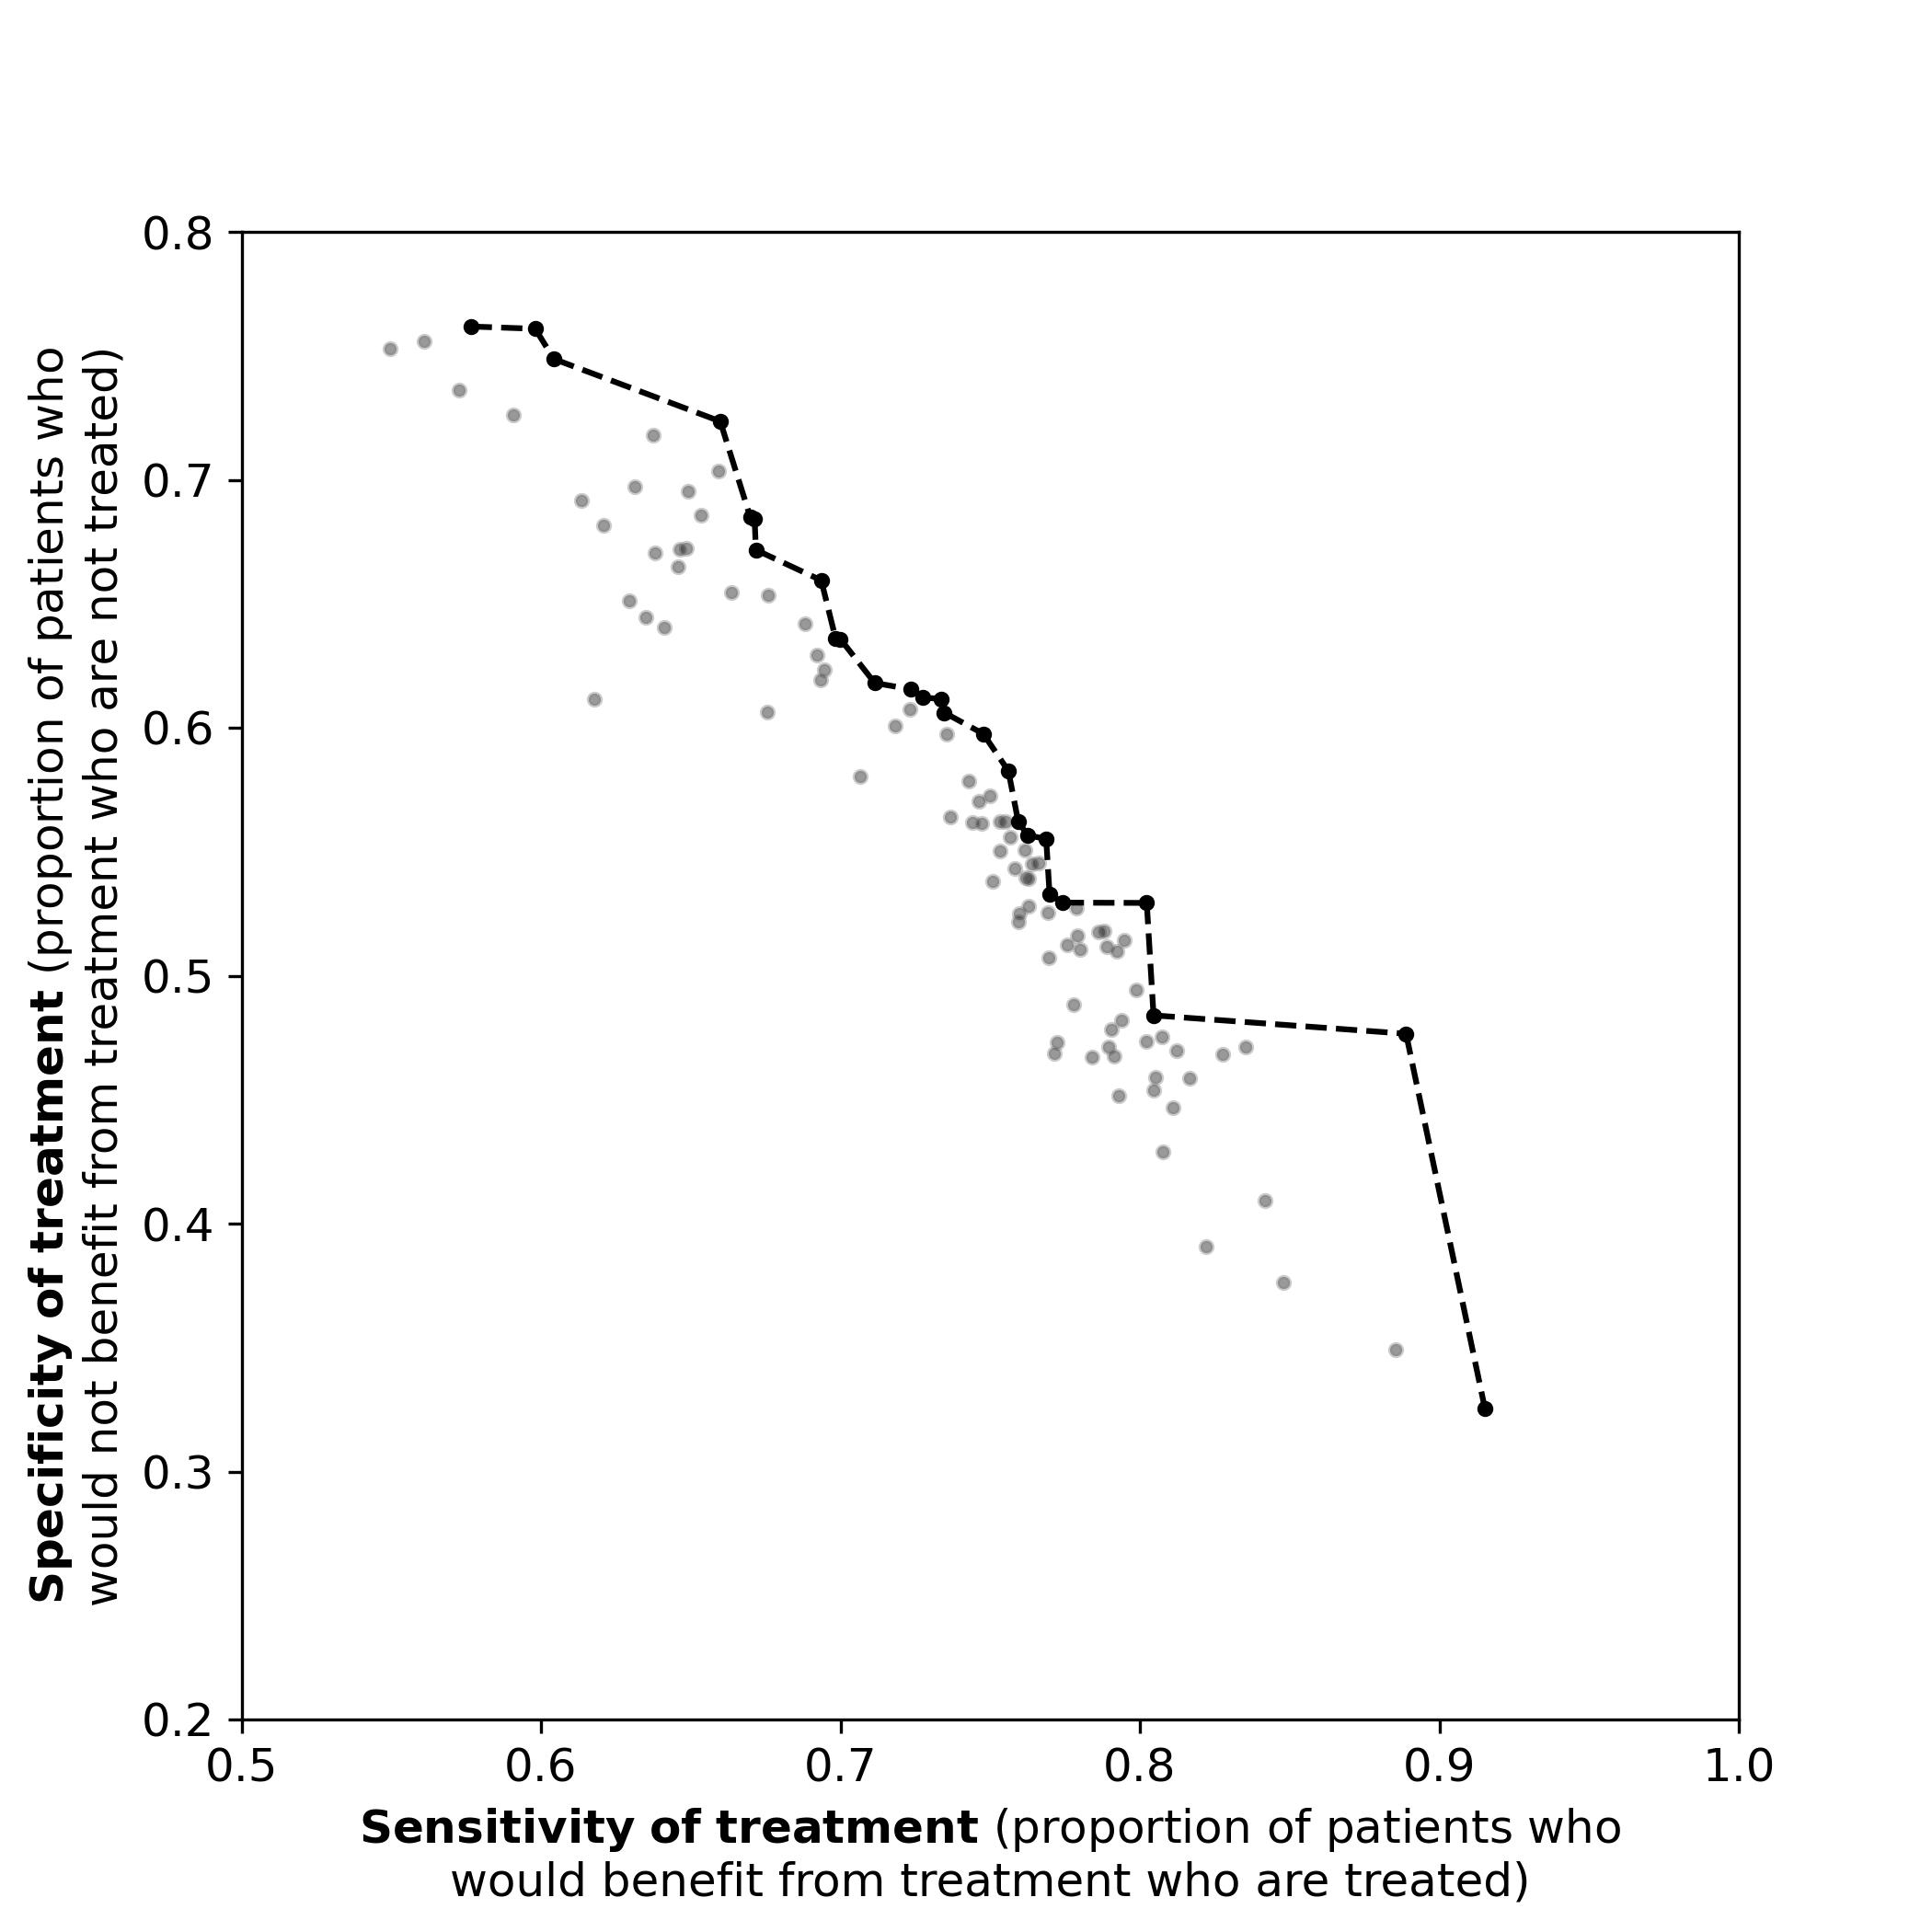
\includegraphics[width=3.5in]{./images/210_xgb_all_data_multiclass_outcome_spec_sens.jpg}}\\ 
    \caption{\textit{Sensitivity} (proportion of patients who were predicted to benefit from thrombolysis who were predicted to receive thrombolysis) and \textit{specificity} (proportion of patients who were predicted \textit{not} to benefit from thrombolysis who were predicted \textit{not} to receive thrombolysis) for each stroke team. The dotted line shows the hospitals on the Pareto front where there are no hospitals that have a better \textit{sensitivity} without a worse \textit{specificity}, or vice-versa.}
    \label{fig:hosp_shap_scatter}
\end{figure}